\RequirePackage[T1]{fontenc}
\documentclass[conference,10pt]{IEEEtran}
\usepackage{amsmath,amssymb,graphicx,url}
\newcommand{\Rone}{\mathrm{R1}}
\newcommand{\Azero}{\mathrm{A0}}
\newcommand{\Btwo}{\mathrm{B2}}
\newcommand{\pct}{\%}
\title{Reachability-Constrained Shared-Crossing Planning for 3D FPGA Routing}
\author{\IEEEauthorblockN{Anonymous submission draft}}
\begin{document}
\maketitle
\begin{abstract}
Vertical connectivity complicates timing-driven FPGA routing because feasible crossings differ across sinks and architectures. We develop a reachability-constrained planner that compares shared and split crossing assignments on a finite terminal hierarchy, then softly guides VTR routing. Controlled experiments separate routing, placement, and toolchain effects across three architectures. On complete dual-baseline cohorts of two to four circuits, timing changes range from a 0.64\% regression to a 1.32\% improvement; larger individual gains coexist with regressions and failures. All ten valid serial timing groups incur overhead. Mechanism analysis exposes sparse delay coverage and motivates a controlled test of the planner's independent contribution.
\end{abstract}
\begin{IEEEkeywords}
3D FPGA, detailed routing, vertical interconnect, dynamic programming, architecture exploration
\end{IEEEkeywords}

\section{Introduction}
Stacking FPGA layers changes the routing decisions that translate architectural resources into performance. A net may share vertical crossings among branches or select separate crossings for critical sinks. Nearby resources may be unreachable through the directed routing resource graph (RRG), and reachable choices may become poor after congestion negotiation or a critical-path change.

Recent tools enable detailed exploration of three-dimensional fabrics. VTR supports 3D architectures, LaZagna generates flexible vertical connectivity, and Escaping Flatland improves the placement flow used to assess these fabrics~\cite{vtr9,vtr9paper,lazagna,flatland}. These advances make it possible to ask a narrower routing question: with the packed netlist, placement, architecture, and timing model fixed, does coordinating crossing choices across a net improve its final routed timing? Answering this question requires distinguishing a routing modification from the benefit of a different placement or a different toolchain.

We investigate a planner that represents legal crossing choices explicitly and compares sharing against splitting within a deterministic hierarchy of remote terminals. The planner combines directed reachability, spatial candidate reduction, criticality filtering, and optional bounded delay queries. Its output is a soft preference used by the existing detailed router. Feasible resources remain available, and the final route is judged by the ordinary routing and timing checks. The implementation is based on a fixed VTR 9 development revision; it is not a new fabric generator or placer.

Our contributions are a finite shared-crossing objective with explicit fallback behavior; fixed-input evaluation across switch-block (SB), output connection-box (CB-O), and hybrid (Hybrid-O) connectivity, separating two placement flows and three baseline identities; and mechanism analysis connecting improvements and regressions to coverage, final resources, changing worst paths, and runtime costs.

The results support conditional timing effects, not a general performance victory. On the complete cohorts used for the paired 3D/2D display, mean routing improvements range from $-0.64\%$ to $1.32\%$, with only two to four circuits contributing to each mean. A single Hybrid-O case improves by $12.96\%$, while another worsens by $11.45\%$. All ten serial groups with three legal paired repetitions are slower than the native baseline. These outcomes make coverage and attribution central to the contribution: a resource-efficient route or a better isolated example does not establish lower critical-path delay across the suite.

\section{Related Work}
VTR provides FPGA architecture and CAD infrastructure~\cite{vtr8}; version 9 added 3D support~\cite{vtr9}. The 3D extensions studied by Boutros et al. connect device models with CAD-level exploration~\cite{third}. We use that infrastructure and retain its detailed router, timing analysis, and legality checks. The new element is a crossing-selection layer above detailed connection search, with a deliberately limited optimization objective.

LaZagna supports architecture generation and evaluation beyond a single vertical-connectivity template~\cite{lazagna}. Its original published VTR 8.1 results and the later VTR 9-code port are different baselines. Neither is interchangeable with the official-source VTR derivative used here. Escaping Flatland addresses partitioning, delay estimation, annealing costs, and moves during placement~\cite{flatland}; our routing comparison instead holds each resulting placement fixed. Its architecture-ranking observations motivate checking rankings, rather than predicting that another routing method must reproduce a reversal.

H3D optimizes bonding-terminal number and positions for face-to-face IC global routing~\cite{h3d}. We borrow the shared-crossing idea, not its geometric model or guarantees. Our finite hierarchy handles directed, prefabricated FPGA resources; it is neither H3D's algorithm nor a global FPGA Steiner-tree solver. Dynamic programming and strongly connected components are established tools, not standalone novelty claims.

\clearpage
\section{Problem Model}
Let $G=(V,E)$ be a directed RRG. Each resource $v$ has capacity $u_v$, physical location and layer, and an associated routing cost. Edges identify actual connections and switches. For each net $n$, source $s_n$ and terminals $T_n$ are fixed by a packed netlist and placement. Detailed routing selects connected legal trees subject to shared capacities, while timing analysis evaluates the resulting circuit. We restrict the planner to two layers and clustered, serial routing.

A crossing candidate $c$ denotes a real vertical entry resource, not a freely placeable via. In the evaluated edge encoding, SB crossings use paired half-nodes and CB-O crossings originate at an output pin. Different CB edges can share the same output resource; counting every edge as an independent via would overstate capacity. A native CHANZ representation is supported separately, but is not silently equated with these edge-encoded resources.

For a remote terminal $i$, candidate $c$ is feasible when a same-layer directed path reaches its entry from $s_n$ and an actual crossing exit can reach $i$ on the destination layer. These conditions certify a single-crossing walk in the full graph. They do not certify a congestion-free route for all nets, a route inside the current search bounding box, or the best possible multi-crossing route. Reverse traversal is an analysis operation only; it never adds edges to the router.

Let $C_i$ be the finite candidate table available to terminal $i$, and let $\alpha_i$ be its routing criticality at initial planning. We use an opening proxy $o(c)$ for source access and prospective resource congestion, and a branch proxy $b_i(c)$ for sink access and criticality. A representative form is
\begin{align}
 o(c)&=d_s(c)+\lambda_o a_c[1+p\max(0,q_c-u_c)],\\
 b_i(c)&=(1+4\alpha_i)d_i(c)+4\alpha_i d_s(c).
\end{align}
Here $a_c$ is accumulated congestion cost, $p$ is the present-cost factor, and $q_c$ includes one prospective unit unless the net already owns the resource. Distances are normalized geometry proxies or supported switch-delay estimates. Partial delay coverage can mix measured opening cost and geometric branch cost.

For hierarchy node $v$, let $L(v)$ contain its terminals. The finite objective is
\begin{equation}
 \begin{aligned}
 S(v)&=\min_{c\in\cap_{i\in L(v)}C_i}\left[o(c)+\sum_{i\in L(v)}b_i(c)\right],\\
 D(v)&=\min\{S(v),D(v_l)+D(v_r)\}.
\end{aligned}
\end{equation}
An unavailable shared choice has infinite cost. At a leaf, only the shared term applies. Opening cost is charged per selected hierarchical group; unrelated groups choosing the same resource do not receive an additional global deduplication credit. Physical same-net sharing is instead represented by the actual route tree. This surrogate omits detailed downstream wire sharing and loading, so lowering it need not lower final circuit delay.

\section{Method}
\subsection{Directed feasibility and candidate reduction}
We query the strongly connected component condensation of same-layer edges, preserving directed reachability. Spatial sampling considers endpoints, interpolated locations, and the net centroid. Feasible candidates are ranked by their proxy costs and diversified across sites; feasible crossings already owned by the net remain eligible. If the spatial sample provides no feasible candidate, the planner scans the crossing table for a usable fallback set. Current occupancy does not by itself exclude a resource, because later congestion negotiation may release it.

The pooled candidates from all eligible terminals form the finite DP table. Each terminal is checked against this pool again, and entries with unavailable measured branch cost are omitted from the surrogate. A candidate introduced by one terminal can serve another. The proposed independent-selection ablation must retain this same table.

\subsection{Finite shared/split planning}
Terminals are recursively divided at the median along the larger spatial extent. At each hierarchy node, the recurrence compares one common crossing with the two child solutions. Induction over the hierarchy proves optimality within these alternatives: each allowed partition either shares at the current node or consists of allowed child partitions. This statement does not cover other hierarchies, excluded candidates, or global capacity coupling. Ties favor a shared group, then deterministic candidate order. Nets with more than 128 eligible remote terminals use independent candidate guidance and increment a fallback counter.

\subsection{Budgeted delay scoring and routing integration}
Delay queries perform bounded exploration and cache endpoint results. The implementation accepts its additive switch-delay proxy only for its supported zero-wire-RC model. A truncated search is not an infeasibility proof. Fully delay-scored terminal choices require enough candidates covered by both forward and reverse searches; otherwise geometric terms remain available. We report query, truncation, cache-hit, and fully scored-terminal counts separately.

The selected configuration uses a static guide: each net is planned once, and the guide is reused on later reroutes. Unpreferred crossing resources receive a nonnegative extra congestion preference, while existing timing-driven search and congestion penalties remain active. A failed guided sink search retries without the guide before ordinary recovery. Static caching bounds repeated planning but may preserve an early decision after congestion or criticality changes. This tradeoff is part of the method, not a claim that all later routing states are optimized.

\subsection{Selective target feedback (development candidate)}
The independently developed candidate Tf retains the frozen R1 initial plan and cost integration, but permits selective guide refresh. VPR first selects a net for native rerouting. Before pruning, we capture its crossing occupancy and actual crossing set; after pruning, VPR supplies the remaining-target set $T_n$. A refresh requires a three-iteration cooldown and either crossing overuse, eligible criticality drift of at least 0.15, or crossing-set Jaccard distance of at least 0.25. Criticality drift remains a net-level trigger; restricting that trigger to targets is a separate, unselected ablation.

The new finite table contains only eligible remote terminals in $T_n$. Static SCC information and valid distance results are reused; congestion prices and candidate assignment are recomputed. Both the old and proposed assignments are evaluated on the current table with the same shared/split objective. For finite old cost, a finite proposal is accepted only if $J_{\rm new}<0.95J_{\rm old}$. An unavailable old assignment may be replaced by a finite one; absence of any eligible target instead permits deactivation of target guides. This exception is an eligibility update, not a cost-improvement claim. Guides and recorded criticalities outside $T_n$ remain unchanged. A membership bitmap makes this preservation check linear in the number of sinks plus targets.

Accepted guides participate in the existing routing transaction and best-route snapshots, so recovery restores the associated guidance state. The method does not force a retained branch to reroute, alter physical switch delays, or replace native congestion negotiation or final STA. Reducing the active terminal set can also bring a high-fanout net below the existing 128-terminal shared-DP limit; this is part of the change, not evidence that every gain comes from avoiding updates to retained branches. Tf remains a development candidate pending broader quality, failure, and controlled runtime validation.

\clearpage
\section{Experimental Setup}
\subsection{Tools, architectures, and comparison identities}
The native baseline A0 and our router R1 derive from official VTR development commit \texttt{0b912334}; R1 adds the planner and graph-encoding integration. Strict serial builds have separate recorded binary identities. B2 is the modern LaZagna port at VTR commit \texttt{5abd3aca}~\cite{modern}, with archived build and compatibility changes. It has been built and exercised under controlled inputs. Its historical version string is not used to infer equivalence with official VTR 9. The original LaZagna VTR 8.1 paper is B1, an external published reference rather than a matched local routing experiment.

We use derived SB, CB-O, and Hybrid-O architectures with a common planar graph and segment mix. Vertical connections retain their generated directions and switch timing. Import checks compare directed connections, switches, and resource semantics between source and native representations. Matching logical capacity does not imply equal area, power, or vertical-interconnect budgets. The modeled wires have zero R/C while switch delays remain; these are architecture experiments, not calibrated silicon predictions.

For each circuit, the registered sizing rule selects the smallest permitted grid side satisfying at most 80\% occupancy for every logical block class. A common size is used across architectures and placement flows. The matched 2D reference preserves logical capacities with a separate near-square layout. Its planar wire-unit inventory differs from 3D by $-0.18\%$ to $+1.87\%$ across the prepared models. It is an architecture/placement denominator, not a fixed-placement routing control. Main measurements use width 100 and ideal clocks, a maximum of 200 routing iterations, disabled failure prediction, a 1800-second route-process limit and a 3600-second placement limit. A 64-GiB address-space cap applies per solver.

\subsection{Placement, selection, and evaluation separation}
P0 is native placement on the paper-packed netlist. P1 executes the paper placement flow, including weighted TritonPart initialization, and repacks to populate criticality information. Packed-netlist semantics are checked against the census. Every A0/R1/B2 routing contrast within a flow uses private copies of the same packed netlist and placement coordinates, with equivalent graph and timing inputs. A P1/P0 contrast changes placement and setup work and is reported separately.

Six training circuits use seed 11: attention\_layer, bnn, eltwise\_layer, gemm\_layer, softmax, and spmv. Fourteen other circuits use evaluation seeds 21, 23, and 25. These circuits had appeared in historical development experiments; the split is fresh for this selection exercise, not evidence of previously unseen benchmark families. Each of four variants---geometry (G), delay (D), criticality (C), and their combination (D+C)---receives eight registered configurations per architecture. All four retain the shared/split DP. Selection prioritizes legal coverage and then circuit-balanced timing on comparable training cases; selected configurations are frozen before evaluation.

\begin{table}[h]
\centering\caption{Frozen selected configurations. $K$ is the candidate target, $\tau$ the criticality threshold, $B$ the per-query settled-node budget. Delay budget is inactive for C.}
\label{tab:config}
\begin{tabular}{lrrrrrr}\hline
Architecture & Variant & $K$ & $\tau$ & $B$ & $\lambda_o$ & Miss\\\hline
SB & C &16&0.80&8192&4&4\\
CB-O & C &8&0.95&1024&4&4\\
Hybrid-O & D+C &16&0.70&4096&16&2\\\hline
\end{tabular}
\end{table}
The held-out main schedule has 168 circuit/seed/architecture cases, including matched 2D cases, with multiple routing roles per case. The separate transferred-width schedule has 12 cases. Fixed-parameter and equally budgeted selected-parameter ablations use seed 21 and P1. Identical immutable configurations can share one execution through explicit role references; reused executions are not independent observations.

\subsection{Validation, metrics, and aggregation}
A result enters a CPD ratio only after VPR FULL checking and the registered independent directed-edge, switch, tree, and node-capacity audit. The independent checker complements rather than replaces VPR: it does not independently establish every terminal-identity or configuration-closure condition. Failed, timed-out, or unexecuted descendant roles remain in coverage accounting. We never insert zero delay for a missing route.

For circuit $j$, we first average the three seed CPDs within each arm. On a complete paired circuit set $S$, we report
\begin{equation}
 I=100\left[1-\exp\left(\frac{1}{|S|}\sum_{j\in S}\log\frac{\bar d_{j,R1}}{\bar d_{j,base}}\right)\right].
\end{equation}
Positive $I$ denotes improvement. The paired 3D/2D display uses the same complete intersection for both denominators. Legal individual pairs outside that intersection still contribute to the separate win/tie/loss counts. Toolchain comparisons may have a different complete set and cannot be subtracted from these means.

Formal runtime uses three serial repetitions of spmv and robot\_rl, both flows, all architectures, and rotated router order. R1-off controls separate algorithm overhead from build differences. A seccomp guard prevents worker-thread creation without ptrace instrumentation. Registered study processes do not overlap, but the shared host is not exclusive. We report router time, route-process time, and setup costs separately. Parallel-sweep durations are mechanism observations, not speedup evidence.

\clearpage
\section{Results}
\subsection{Timing, failures, and the three baselines}
Table~\ref{tab:main} reports the complete dual-baseline cohorts. Hybrid-O has small positive means in both flows; SB changes sign across flows, and CB-O is unchanged against A0 at reported precision. The 2D comparison can differ substantially because it includes a different physical layout and placement. For example, CB-O/P0 improves by 3.05\% against matched 2D while showing zero routing improvement against its own 3D A0. This is not a routing speed or timing gain attributable to R1.

\begin{table}[h]
\centering\caption{CPD improvement (\%). Parentheses give the matched 2D comparison on the same $n$ complete circuits. Each panel registers 14 circuits and 42 seed samples. W/T/L counts cover all legal R1/A0 seed pairs, not only the complete dual cohort.}
\label{tab:main}
\begin{tabular}{llrrr}\hline
Fabric & Flow & $n$ & vs. 3D (vs. 2D) & W/T/L\\\hline
SB & P0 &3&$-0.64\;(-7.17)$&9/4/10\\
SB & P1 &4&$+0.41\;(+0.89)$&7/6/11\\
CB-O & P0 &2&$0.00\;(+3.05)$&0/11/0\\
CB-O & P1 &2&$0.00\;(+4.28)$&0/12/0\\
Hybrid-O & P0 &3&$+1.32\;(+0.35)$&7/9/7\\
Hybrid-O & P1 &4&$+1.08\;(+1.05)$&11/9/4\\\hline
\end{tabular}
\end{table}

\begin{table}[h]
\centering\caption{Main held-out role outcomes: legal/failed/timeout, 42 roles per cell. Failed includes registered failures and unavailable descendants, not only router nonconvergence.}
\label{tab:coverage}
\begin{tabular}{llrrr}\hline
Fabric&Flow&A0&R1&B2\\\hline
SB&P0&23/11/8&23/10/9&24/10/8\\
SB&P1&24/8/10&24/8/10&24/8/10\\
CB-O&P0&11/27/4&11/27/4&11/27/4\\
CB-O&P1&12/27/3&12/27/3&12/27/3\\
Hybrid-O&P0&24/10/8&23/10/9&24/9/9\\
Hybrid-O&P1&24/12/6&24/11/7&24/12/6\\\hline
\end{tabular}
\end{table}
Failures are substantial, especially for CB-O. The 756 main 3D roles yield 354 legal routes, 280 routing failures, 121 timeouts, and one allocation failure under the registered limit. Matched 2D contributes only 17/42 legal references. Across evaluation including ablations and transferred width, 581/1206 roles are legal, 455 fail, and 170 time out; reuse gives 1136 unique attempts (552/423/161). These are execution counts, not independent circuits. Failed routing logs can contain positive CPDs; such values are excluded.

Against modern LaZagna B2, the R1 mean CPD improvements are $+0.67\%/-1.60\%$ for SB P0/P1, $-0.67\%/+0.57\%$ for CB-O, and $+1.61\%/-2.27\%$ for Hybrid-O. The respective complete-circuit counts are 7/8, 2/2, and 6/8. These are toolchain contrasts on matched inputs. They do not establish that the planner causes every R1/B2 difference, particularly where R1 and A0 tie.

For B1, the original LaZagna paper reports normalized CPDs of 0.821, 0.819, and 0.809 for 100\%, 66\%, and 33\% SB connectivity, respectively, relative to its own 2D reference~\cite{lazagnav1}. Those architectures, circuits, and denominators do not match this experiment. We retain these published values as context and leave the direct R1/B1 ratio undefined. The newer tool port and historical source reproductions do not substitute for the author's published measurement.

The largest same-sample dual gain is Hybrid-O/P0, clstm\_like.small, seed 23: 12.96\% against A0 and 10.54\% against matched 2D. It coexists with an 11.45\% regression for clstm\_like.large, seed 23, in the same architecture and flow. Across SB/P0, robot\_rl seed 21 worsens by 13.30\%. Extremes illustrate sensitivity; none replaces a mean or a failure denominator.

\subsection{Runtime cost and architecture ordering}
All ten R1/A0 groups with three legal serial repetitions incur router overhead, with median ratios from 1.129 to 3.382. The corresponding route-process ratios are 1.047--1.313. Two robot\_rl/CB-O groups lack legal paired repetitions and remain missing rather than neutral. Observed median setup spans 13.59--71.25 s, including 0.84--6.04 s of partition work where applicable. P0 reuses census packing whereas P1 repacks; these are flow-specific costs, not equal-work end-to-end speedups.

The same-build R1-off control also shows overhead in all ten complete groups: R1/R1-off spans 1.180--3.327 for router time and 1.015--1.334 for process time. Against B2, these ranges are 0.906--4.214 and 0.910--1.267; only one and two groups, respectively, are faster. These toolchain differences do not establish overall acceleration.

Only conv\_layer\_hls belongs to the complete intersection across all three architectures and both routing/placement choices. On this circuit's three-seed means, all four combinations rank CB-O, then SB, then Hybrid-O; the strict reversal count is zero. Individual seed rankings change, however: P1 ranks SB first at seed 21 and Hybrid-O first at seed 25, for both A0 and R1. With this limited intersection, neither a general best architecture nor a ranking reversal is supported. Architecture exploration needs robust coverage and a credible physical comparison, in addition to a successful search method.

\begin{figure}[h]
\centering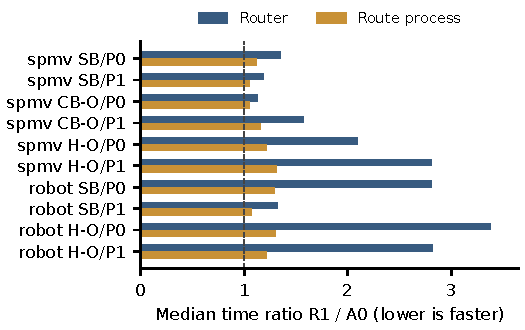
\includegraphics[width=\columnwidth]{figures/strict_runtime.pdf}
\caption{Strict serial timing: all ten complete groups exceed unity. Two registered robot\_rl/CB-O groups have no legal three-repeat pair and are omitted from ratios, not from coverage.}
\label{fig:runtime}
\end{figure}

\clearpage
\section{Mechanism Analysis}
\subsection{Coverage is narrower than the algorithm's name}
The frozen CB-O threshold of 0.95 selects few remote terminals. Across its legal main runs, the mean selected-terminal fraction is 0.142\% for P0 and 0.0143\% for P1; all legal R1/A0 CPDs tie. Sparse guide application is consistent with this lack of a final timing effect, but the counters alone do not establish that a lower threshold would help. A broader guide can also increase work or redirect routing adversely.

Hybrid-O enables delay estimation, yet complete forward/reverse coverage is rare. Its legal P0 runs fully score 32 of 44,064 eligible terminals in aggregate; P1 scores 60 of 43,119. All 32,941 P0 and 46,650 P1 recorded endpoint queries hit their exploration cap. Truncation does not imply an empty query: settled entries remain useful, and measured source costs can affect choices that fall back for branch scoring. The data expose a mismatch between the configured budget and the candidate sets, rather than proving that delay-aware optimization is intrinsically ineffective.

\begin{table}[h]
\centering\caption{Mechanism cases, Hybrid-O/P0, seed 23, W100. Resource values are audited final-route counts; timing costs are observed sweep diagnostics.}
\label{tab:mechanism}
\small\setlength{\tabcolsep}{3pt}
\begin{tabular}{lrr}\hline
Quantity&small CLSTM&large CLSTM\\\hline
CPD A0 $\rightarrow$ R1 (ns)&7.1478 $\to$ 6.2215&7.0737 $\to$ 7.8835\\
SB pairs A0 $\rightarrow$ R1&53 $\rightarrow$ 40&51 $\rightarrow$ 52\\
CB sources A0 $\rightarrow$ R1&1159 $\rightarrow$ 1164&2873 $\rightarrow$ 2870\\
Planar length A0/R1&227162 $\rightarrow$ 227088&629142 $\rightarrow$ 629368\\
Eligible / remote&530 / 3902&1233 / 10863\\
Delay-scored / eligible&2 / 530&2 / 1233\\
Queries / capped&808 / 808&1778 / 1778\\
Planning time (s)&28.73&106.13\\
Router A0 $\rightarrow$ R1 (s)&5.84 $\rightarrow$ 34.78&17.26 $\rightarrow$ 126.24\\
Iterations A0 $\rightarrow$ R1&26 $\rightarrow$ 26&24 $\rightarrow$ 29\\\hline
\end{tabular}
\end{table}

\subsection{An improvement with a different critical path}
For clstm\_like.small, the planner selects 530 of 3902 remote terminals, forms 372 groups, and records no empty-candidate, high-fanout, or guided-search fallback events. The final route uses thirteen fewer SB pairs but five more CB crossing output sources. Planar length falls by only 74 units, or about 0.033\%. The observed CPD gain therefore accompanies a change in route topology rather than a large reduction in total wirelength.

The saved A0 worst path runs through a multiplier in an inverse-transform block. Under R1, the worst path instead lies in an elementwise subtraction block; the start and end registers both change. Its reduced worst delay shows that the overall routing perturbation improves this sample. However, the two saved reports describe different paths, so their component delays cannot be subtracted as if they measured the same connection. In particular, they do not identify which chosen crossing relieved the original worst path. A connection-level causal account would require matched path traces or an additional instrumented control.

Only two eligible terminals receive complete delay scoring. The observed improvement consequently supports the whole selected configuration, not a claim that the bounded delay estimator or DP alone caused it. Planning consumes 28.73 seconds out of 34.78 reported routing seconds, approximately 83\%. The same 26 negotiated-congestion iterations do not imply equal work per iteration. Caching removes repeated planning but does not remove its initial cost.

\subsection{A degradation despite similar resource use}
For clstm\_like.large, CPD increases from 7.07372 to 7.88347 ns. The final route uses one additional SB pair, three fewer CB crossing sources, and 226 more planar-length units, about 0.036\%. These small changes in aggregate resources fail to predict the 11.45\% timing degradation. The worst path changes from one multiplier/register chain to a different inverse-transform multiplier path. The saved reports again support a bottleneck change, not a matched-edge delay decomposition.

The planner forms 938 groups from 1233 eligible terminals, but only two receive complete delay scoring. It records no guided-search, high-fanout, or empty-candidate fallback. Thus fallback activation is not an explanation for this regression. A feasible, cached guide can simply steer congestion negotiation toward a worse final critical path. Planning takes 106.13 of 126.24 router seconds, approximately 84\%, and routing needs 29 iterations instead of 24. This case exposes both proxy mismatch and substantial setup cost.

Pairing final connections by net name, pin index, and identical SOURCE/SINK resource IDs yields an additional distinction. In the large case, mean switch delay across all 10,863 remote connections falls from 1.92973 to 1.87781 ns (2.69\%): 3485 improve, 4617 tie, and 2761 regress, despite worse CPD. The small case has 626/2735/541 outcomes across 3902 remote connections, with a 1.65\% mean improvement. These audited zero-RC switch sums exclude local logic delays and do not isolate a planner component. Better average interconnect quality can coexist with a worse worst path.

\subsection{What final resource counters establish}
Independent route audits establish the final SB-pair and CB-source occupancies reported above. The \texttt{guided\_paths} and \texttt{preferred\_paths} logs instead count routing events across iterations, including reroutes. For the favorable case their final values are 3657 and 2023; they are not a 55\% final-route adoption rate. No frozen per-connection final-guide trace is available to compute that rate. We therefore distinguish final resource use, cumulative guide events, and causal resource selection. Their identities must not be inferred from similar aggregate totals.

\clearpage
\section{Sensitivity, Attribution, and Limitations}
\subsection{Scoring ablations and partition balance}
The four scoring variants are compared with configuration 0 fixed and with equal eight-configuration training budgets. On the joint P1/seed-21 Hybrid-O cohort of four circuits, fixed G, D, C, and D+C improve CPD over A0 by 5.63\%, 4.25\%, 0.38\%, and 0.38\%, respectively. After separate selection, the values are 5.63\%, 2.51\%, $-1.89\%$, and 3.29\%. Individual legal coverage differs: selected D has 4/14 legal pairs and selected D+C has 8/14. The common-cohort mean and broader coverage describe different properties. These results do not support monotonic benefit from adding scoring terms, and all arms still contain DP.

A registered balance sensitivity study compares literal partition argument 0.03 with a relative-3\% interpretation, argument 1.5 for two equal target partitions. Across four circuits, three architectures, two widths, two placement arms, and three routing roles, 130 of 144 roles are legal, 12 fail, and two time out. Independent weight audits satisfy their respective bounds in 18/24 literal and 24/24 relative placements. Training and evaluation remain separate. At W100, the two-circuit held-out Hybrid-O cohort improves by 0.763\% for R1/A0 under the literal arm and 1.065\% under the relative arm. Nevertheless, moving from literal to relative worsens A0 by 0.911\% and R1 by 0.605\%. A better routing ratio therefore need not mean a better total flow. For CB-O, the one legal held-out pair improves by 1.330\% under the placement change, equally for A0 and R1: this is a placement effect.

\subsection{DP attribution in the frozen evaluation}
The current \texttt{candidates} mode is not an adequate DP-off control. It changes guide lifetime and retains multiple independent preferences, while the DP commonly assigns a singleton. The frozen v13 evaluation did not execute an independent top-1 control. The post-registration development experiment below implements two arms sharing candidate sampling, the pooled feasible table, scores, delay queries, congestion state, and static cache lifetime. Arm I selects each terminal's minimum opening-plus-branch-cost candidate independently; Arm S applies shared/split DP to the same table. Both produce singleton guides on the supported DP population. Existing high-fanout and empty-table fallback behavior remains common.

The isolated development snapshot adds one selector after table construction. Validation must reproduce frozen DP-on routes and CPDs, verify both solvers on enumerated small tables, and check cache behavior. First-plan table hashes verify equality; later trajectory differences are guidance outcomes.

The proposed diagnostic pilot uses spmv/SB/P0/seed11, small and large CLSTM/Hybrid-O/P0/seed23, and conv\_layer\_hls/CB-O/P1/seed21: selected training, improved, regressed, and tied cases. Eight primary runs plus timing repeats on two cases give sixteen runs, capped at eight solver-hours plus four build/check hours. This unexecuted twelve-hour design has no sweep or blind-test claim.

\subsection{Fixed-placement width diagnostic}
The registered fixed-placement diagnostic completed all 24 cases and 144 roles: 125 legal, 13 failed, and 6 timed out. For selected R1, 19 of 24 four-route width interactions are complete; five are incomplete. The interaction $(R1/A0)_{300}/(R1/A0)_{100}$ is below, equal to, or above one in 5, 11, and 3 cases, respectively. Each split contains two circuits at one seed. Earlier 1.39\% and zero-improvement studies used different graphs and placements; width alone is not an established explanation. This diagnostic changes connectivity and possible congestion together, so it cannot isolate congestion as the sole mechanism.

\subsection{Limits of inference and implications for exploration}
Dual-baseline cohorts cover only two to four of fourteen circuits. Architecture-dependent missingness prevents all-suite claims; three seeds do not establish broad significance, and prior exposure limits independence. Logical-capacity and planar-graph matching do not equalize silicon area, power, or via budgets. Ideal clocks and zero-wire-RC models limit technology-level inference.

Mechanistic uncertainty also remains. The shared/split recurrence is implemented and independently checkable, but the present scoring ablations do not isolate its contribution. Sparse delay-query coverage, a fixed hierarchy, candidate truncation, static criticalities, and lack of global congestion coupling can all limit the surrogate. Candidate-table reuse and more targeted delay queries are plausible optimization directions; they were not measured in the frozen evaluation, and the separate development study below tests them. The strict timing results already rule out describing the current implementation as a general acceleration.

Architecture exploration should report legality, timing, resource use, and cost together. A few improved samples cannot establish a general architecture ranking; no reversal is an acceptable outcome.


\section{Post-registration Development: Candidate-level Delay}
This section reports development after the frozen v13 evaluation; it does not replace that experiment or its denominator. We test whether sparse measurements become more useful when the all-or-nothing terminal scoring gate is removed. For each endpoint and query direction, settled candidate distances are normalized by the same graph-derived delay unit. Missing distances use a geometric proxy multiplied by an endpoint-local scale: the median observed delay-to-proxy ratio, shrunk toward one with eight prior samples. Measured distances themselves are not shrunk. With no observations, geometry remains the explicit fallback. Reverse queries remain enabled even if the bounded source query returns no crossing, because reverse-only information now affects candidate scores.

The hypothesis is tested at the frozen Hybrid-O settings ($K=16$, query budget 4096, opening weight 16, miss weight 2, minimum criticality 0.7), initially on spmv and softmax with P0, W100 and seed 11. We first require the new binary with the feature disabled to reproduce the frozen R1 route body, CPD, wirelength and iteration count. All valid new routes additionally undergo the existing directed-edge, switch, tree and capacity audit; its original scope limitations remain. These are previously observed development circuits, not a new blind evaluation. The initial two-circuit paired experiment passes the default-off reproduction gate and all four new routes pass FULL and the registered independent audit. On spmv, calibrated partial scoring changes CPD from 7.04599 to 7.26887 ns (3.16\% worse than R1), while softmax remains at 8.97575 ns. The circuit-geometric mean CPD increases by 1.57\%; this small development result does not justify promoting the scorer. At unchanged query counts (148 and 69), all 107 and 108 eligible connections, respectively, have at least one candidate informed by measured distance, whereas the legacy complete-bilateral count is zero. These coverage definitions differ: partial information availability does not mean complete measurement or critical-path improvement. spmv uses zero rather than one SB net-occupancy unit, while CB occupancy remains 967, again showing that aggregate crossing counts do not predict CPD. Planning/process times are recorded in the artifact, but these single development measurements establish no speedup. Physical switch delays, STA and the native congestion mechanism are unchanged.

The second hypothesis is a bounded soft preference expressed in timing-cost units, weighted by measurement reliability and connection criticality. The third is selective guide reassignment only for nets already chosen for rerouting, triggered by congestion or substantial timing/path changes, with reuse of static indices and hysteresis. The timing-cost control is implemented with amplitude 0.25 graph delay units, multiplied by the measured-side fraction of the selected preference and by connection criticality. It is restricted to the ordinary setup-timing search, leaves physical Tdel unchanged, and is tested separately from the scorer below. A same-table independent top-1 control is also implemented and has passed 250 small-table enumeration checks. Selective dynamic reassignment is implemented as a separately gated development candidate; the completed routing, forced-rollback and component-ablation results are reported below. Combinations require separate validation first. Formal runtime claims require fresh, serial, rotated repeats in the same environment; development and historical times do not establish speedup.

The separate F/H/N/G development batch contains eight valid new runs. All F/H and F/N finite-table fingerprint sequences match (88 plans for spmv, 43 for softmax), and both F routes reproduce frozen R1. On spmv, H reduces CPD to 7.04234 ns (0.052\% versus R1) and iterations from 19 to 15, but remains slower in CPD than A0 at 7.03470 ns. N and G retain R1's CPD, with 15 and 17 iterations respectively. All four arms have softmax CPD 8.97575 ns and 13 iterations. The two-circuit geometric CPD improvement of H over R1 is only 0.026\%, insufficient to select a stable method. These observations motivate broader development and final guide-adoption tracing, while leaving targeted uncertainty-driven queries as open implementation work; the subsequent sections report completed dynamic-update validation.



\subsection{Development expansion and selective feedback candidate}
The F/H/N/G expansion on eltwise\_layer, bnn, gemm\_layer and attention\_layer is complete, independently audited and input-sealed. Together with spmv/softmax, all six declared development circuits remain in the denominator. Five are legal under every arm; attention fails under all four, as under A0/R1. H improves one legal circuit, ties one and worsens three: its circuit-geometric-mean CPD change is 3.391\% worse, with a 15.928\% worst regression on eltwise. N ties four and worsens eltwise by 4.283\% (0.842\% worse geometrically); G ties three and worsens two (2.022\% worse geometrically, 10.463\% worst). gemm F/H/N/G CPDs are 13.1564/13.2393/13.1564/13.1564 ns. These matched-parameter development comparisons support retaining the existing shared assignment and delay control as references; they do not justify promoting the tested H preference. No success-rate improvement is established, and the failed circuit is not omitted. Detailed case-level values and physical-resource metrics remain in the sealed observations.

A separate update candidate examines only nets already selected by VPR for rerouting. Recommended crossing overload, remote criticality drift of at least 0.15, or crossing-set Jaccard change of at least 0.25 triggers consideration, subject to a three-iteration cooldown. Static SCC and endpoint distance caches are reused. Existing candidates are retained and rechecked for feasibility. The old and proposed assignments are evaluated on the same current finite table and hierarchical opening-charge rule; a proposal with a complete finite-cost prior assignment requires more than 5\% surrogate improvement. If new eligible pins leave that prior assignment incomplete, its cost is infinite and a finite feasible replacement may be accepted; this is distinguished from finite-cost improvement. If no remote terminal remains eligible, obsolete guides are explicitly deactivated, which is not counted as an objective-improvement claim. High-fanout fallback is retained. Prices currently emphasize crossing entries, so downstream CB congestion may remain poorly represented.

Existing full-tree transaction restoration is extended to guide and feedback state. A final diagnostic snapshots guides when VPR saves its best routing, then observes adoption against the restored final route trees. The independent trace checker reconstructs each guided pin's source, sink and actual crossing identities from the emitted route. Recorded planned criticality is distinguished from final STA criticality. The fixed-assignment cost evaluator passes 4,280 comparisons against independent hierarchical-plan enumeration; cooldown, margin and trace-reconstruction tests also pass. The completed two-circuit F/U/forced-rollback-X pilot adds six routes passing FULL, graph audit, and final-guide audit; F reproduces R1 and each X case exercises one guide rollback. X is a transaction diagnostic and its QoR is not treated as an algorithm result. U leaves spmv and softmax CPD and iteration counts unchanged. spmv has 37 refresh attempts: nine accepted deactivations, four accepted replacements of incomplete prior assignments, and 24 rejected equal finite-cost proposals. softmax has ten attempts: six deactivations, two incomplete-prior replacements, and two equal-cost rejections. Neither case accepts a finite-to-finite cost improvement. On the common guided-pin populations, adoption is unchanged (78/104 for spmv and 94/108 for softmax); larger overall adoption counts reflect different guided populations. spmv planning time rises from 3.280 to 5.562 s in this development run, without a CPD gain. In the unchanged-parameter expansion, audited eltwise\_layer U improves CPD from 6.96208 to 6.37264 ns (8.47\%) and reduces iterations from 46 to 34. Among 150 attempts, four finite-cost improvements, 40 incomplete-prior replacements and 43 deactivations are accepted. Common-pin adoption changes from 100/140 to 102/140, with seven losses and nine gains. Planning increases from 4.906 to 8.698 s and full process time from 32.429 to 34.982 s in this development measurement, so this quality benefit is not a speedup. attention\_layer F/U both fail at 200 iterations, and unchanged U on bnn passes all audits; the single positive circuit does not justify freezing. Whether overload triggers observe resources absent from the entry-based pricing remains a hypothesis to test.


\subsection{Prototype for reusing candidate-query work}
A standalone query prototype retains one endpoint's Dijkstra frontier across changing candidate-target requests and stops when the requested terminals are settled. All calls share one cumulative settlement budget; tentative labels are never reported as measured distance. Per-state node and heap-entry bounds stop further work on memory exhaustion while preserving previously settled results. Across 500 random directed graphs, 2,000 terminal-distance checks match the existing unbounded reference search, including zero-weight edges, cycles and unreachable goals. A synthetic two-request example reduces settlements from 10 with restarts to 7 with reuse. This is a mechanism check, not an RRG speedup or routing-quality result. A separate cache prototype adds a fixed number of live frontier slots, a bounded non-evicting endpoint work ledger, and an aggregate work cap. Eviction does not replenish an endpoint budget; a full ledger declines new keys. These limits bound container entry counts, not allocator bytes, and process memory guards remain necessary. Ten thousand alternating requests check exact returned distances and work accounting under eviction. Candidate/criticality/uncertainty scheduling and router integration remain pending. The prototype is isolated from all running and queued router binaries.

The prototype is also checked on the frozen spmv Hybrid-O W100 RRG (1,028,568 nodes and 4,994,132 edges). Eight previously routed cross-layer connections selected by ascending net identifier yield 16 directional requests over 11 distinct endpoint/direction pairs. An independent full same-layer Dijkstra records crossing costs on physical edges. All ten bounded-query measurements match this reference; six budget-limited requests remain unknown despite reachable targets. Resumption uses 11,510 settlements versus 31,187 when rebuilding every request. This is not a comparison against R1's existing endpoint cache. Targets taken from final routes are diagnostic and do not define a prospective candidate policy. Two live frontier slots preserve all ten measurements at 11,510 settlements on this request sequence, while one slot yields nine measurements and 12,312 settlements because rebuilding consumes the remaining endpoint allowance. This illustrates an eviction/coverage tradeoff, not a general minimum cache size. Target stopping alone does not change the Dijkstra expansion order: under an identical per-endpoint budget, it can avoid work but cannot by itself increase exact-distance coverage. Candidate-directed search or evidence-based work redistribution therefore remains necessary. No routing-quality or runtime benefit is inferred from these checks.


\subsection{Candidate-directed bidirectional query candidate}
A further query candidate searches from both the endpoint and a requested crossing in the correctly reversed directed graph. A meeting path remains an upper bound until the sum of frontier minima proves optimality. Both fronts consume one cumulative endpoint/direction settlement allowance across successive candidate requests. Independent Floyd--Warshall checks cover 20,000 full and 20,000 bounded random directed source/target pairs. On the same 16 real-RRG diagnostic requests, the original cached endpoint search measures ten targets using 45,056 settlements; the candidate-specific search measures all sixteen using 2,352. Every measured distance agrees with the independent physical-edge reference. Both methods retain a 4096-settlement allowance per distinct endpoint/direction. This is a diagnostic work-count comparison on targets taken from completed routes, not prospective QoR or wall-time evidence.

The compiled router candidate instead requests up to $K$ diverse feasible crossings selected from information available during planning: geometry, current congestion, SCC feasibility and already known distances. It retains the partial-delay scorer's calibrated estimates for unknown distances, caches exact candidate measurements, and preserves cumulative endpoint work accounting. One temporary bidirectional frontier is bounded by label and heap-entry limits and released after each request. The completed F/M/T pilot contains six audited legal routes: F reproduces R1, M reproduces the prior partial-scoring control, and T changes candidate-query measurements. Timing guidance and feedback refresh are disabled in this pilot. T recovers spmv CPD from M's 7.26887 ns to R1's 7.04599 ns, but takes 21 rather than 19 iterations; softmax remains at 8.97575 ns and 13 iterations. Pool-level bilateral measurement counts fall from M's 235 to 221 for spmv and from 228 to 39 for softmax. T uses 584,851 versus 606,208 settlements for spmv and the same 282,624 for softmax, while planning time increases from 3.169 to 3.591 s and from 4.186 to 4.412 s. These development measurements do not establish acceleration. The known-route-target diagnostic therefore does not generalize directly to prospective candidate pools. One difficult target may consume the remaining endpoint allowance, and one-shot queries discard work not retained as exact candidate values. A new Q control caps each candidate at 256 settlements while preserving the 4096 endpoint total, and adds selected-guide measurement counters; its eight-run paired experiment has completed with all route and final-guide audits and input seals passing. This fixed allocation is not yet criticality/uncertainty adaptive, and the Q batch does not establish a general quality gain. Its audited spmv result retains R1 CPD with 17 iterations; selected-guide bilateral measurement counts are M/T/Q=33/59/32 out of 107 guided pins. T therefore increases selected bilateral coverage despite decreasing pool coverage, while fixed Q slices do not improve that selected coverage. Q spends 506,369 settlements for spmv. For softmax, all arms retain 8.97575 ns and 13 iterations, selected bilateral counts M/T/Q are 43/19/16 out of 108 pins, and Q uses 261,155 settlements. Fixed Q slices improve neither circuit's CPD over R1 and do not establish a formal timing benefit.


\subsection{Critical-path migration and unguided planar connections}
Existing worst-setup reports reveal why local crossing counts alone are insufficient. We bind reported atom drivers and sink-cluster locations to the fixed packed netlist, placement, and emitted route, then compare identical physical SOURCE/SINK connections. All selected routes passed FULL and independent graph audits. Switch-delay sums use the verified zero-RC model and exclude intra-cluster logic/local delays; they are not substituted for final STA. The report provides only the worst path, and its rounded increments do not identify every critical connection.

For spmv, partial scoring improves a crossing connection on the original worst path from 1.17249 to 0.99430 ns, yet a RAM-to-multiplier connection on the new worst path increases from 0.84934 to 2.70760 ns. The latter net has one sink and no cross-layer sink, so it receives no direct crossing guide. For eltwise\_layer, both F and H worst paths contain only same-layer connections. On a 132-sink net with no remote sink, the connection to F's critical sink changes from 4.00838 to 0.84934 ns under H, while a different connection to H's critical sink changes from 1.03517 to 4.20948 ns. The selected critical endpoint therefore migrates; H's longer logical path is not evidence that routing changed the logic. These observations establish indirect route changes on unguided nets, but do not isolate the responsible congestion event. They motivate tracking planar-connection tails alongside guided-pin adoption, rather than treating greater delay coverage or fewer crossings as sufficient evidence of timing improvement. Exploratory full connection pairing retains identical net/pin indices and SOURCE/SINK RR identities, with no unmatched connections in the examined pairs. For eltwise H, 1,460 of 18,275 connections in entirely planar nets worsen by more than 0.1 ns even though their mean delta is slightly negative; the 99th-percentile additive regression is 1.301 ns. For bnn H, the mean cross-layer connection delay improves by 0.074 ns while same-layer connections in mixed nets worsen by 0.149 ns on average. These are physical delay distributions, not STA criticality-weighted or circuit-balanced CPD results.


\subsection{Attributing and reducing planning overhead}
An instrumented eltwise pilot separates mutually exclusive initial and refresh planning phases. Inclusive SCC-closure miss time is reported separately and must not be added again to those phase totals. Under U, 372 closure misses consume 7.536 s of 8.447 s inside the fast planner (89.2\%), whereas assignment solving consumes approximately 2.21 ms. Replacing per-query hash sets with generation-stamped visitation preserves sorted closures exactly. Twenty thousand independent original-graph BFS checks and explicit epoch-wrap tests pass. The resulting O arm reproduces U's complete route body, candidate-table and refresh-decision sequences, final guides, CPD and iteration count. All three pilot routes pass FULL, independent graph and final-guide audits, with sealed paired inputs.

\begin{table}[t]
\centering\caption{Instrumented eltwise development observation. Concurrent single executions; not formal speedup evidence.}
\begin{tabular}{lrrrr}
\hline
Arm & CPD (ns) & Iter. & Plan (s) & Process (s)\\
\hline
F & 6.96208 & 46 & 5.096 & 31.983\\
U & 6.37264 & 34 & 9.095 & 35.542\\
O & 6.37264 & 34 & 5.566 & 32.778\\
\hline
\end{tabular}
\end{table}
O retains U's 8.47\% CPD improvement on this circuit while reducing extra planning work; its full process remains slightly slower than F in this observation. Independent bnn O equivalence confirmation has passed all audits; rotated same-environment timing remains pending. The completed attention F/U comparison fails for both arms at 200 iterations and provides no success-rate recovery.

A diagnostic of the saved spmv RRG identifies extensive common closure structure: distinct endpoints in the same layer and direction share 139,245 SCCs. A subsequent opt-in candidate caches complete closures of at most eight large SCCs, with a shared 4,194,304-entry storage bound across directions and immutable allowed masks. Exact traversal merges cached suffixes; rejected cache insertions retain the original exact traversal. Twenty thousand independent BFS comparisons and eleven real-RRG endpoint comparisons pass, including tight capacity, both directions, overlapping closures and reconfiguration. The real diagnostic stores 556,980 entries. These standalone checks establish exactness on the tested graphs but do not establish prospective QoR or formal runtime improvement. Transient traversal/union space and mask storage are additional to the cache-entry bound and remain subject to process memory guards.

The audited eltwise U improvement also retains connection-level regressions. With identical net/pin and SOURCE/SINK RR identities and zero unmatched pairs, 2,837 of 18,275 connections in entirely planar nets worsen by more than 0.1 ns; the 99th-percentile additive regression is 1.308 ns despite a mean improvement of 0.016 ns. Same-layer pins in mixed nets improve by 0.091 ns on average, while cross-layer pins worsen by 0.022 ns on average. Thus the CPD benefit is not a uniform connection benefit and cannot be explained solely by mean cross-layer delay. These are exploratory physical-delay tails, not final STA criticality.

The completed bnn F/U comparison preserves 13.4216 ns CPD and reduces iterations from 35 to 19, yet planning increases from 261.885 to 336.824 s and full process time from 532.741 to 598.971 s. Among 497 refresh attempts, five finite-cost improvements, 27 incomplete-prior replacements and 303 guide clearings are accepted. Common guided-pin adoption changes from 778 to 777 out of 1,013. Thus fewer iterations and accepted updates do not suffice to establish acceleration or greater adoption.

Across six registered full-feedback development circuits, five are legal under both U and R1: one improves and four tie, with a circuit-geometric-mean CPD improvement of 1.754\%. Attention fails for both and remains in the denominator. Relative to A0, the five legal pairs contain three improvements, one tie and one regression; the geometric-mean improvement is 8.853\%, and the worst regression is spmv at 0.1605\%. The gemm execution uses the same full-feedback quality policy with exact compact closure optimization; its static control exactly reproduces R1. These are single-seed, previously seen development circuits, not independent generalization or success-rate improvement. Formal matched timing is pending.

A subsequent four-arm eltwise experiment validates the shared-closure candidate S in the router. All routes pass FULL, independent graph and final-guide audits and input sealing. S exactly preserves U's route body, costs/assignment-table sequence, refresh decisions and final guides, retaining 6.37264 ns CPD and 34 iterations. In this batch, F/U/O/S planning times are 4.936/8.870/5.446/1.537 s and full process times are 32.375/35.185/32.128/28.321 s. S retains 556,980 cached component entries and reduces 372 inclusive closure misses to 0.086 s; total planning includes cache construction. These concurrent instrumented development measurements motivate the larger-graph confirmation reported below, but are not formal acceleration evidence. S changes exact feasibility-query work rather than the U quality mechanism; its route-quality evidence is therefore the same as U's on this verified case.


\subsection{Bounded lossless closure encoding and residual failure scope}
The bnn O/S runs pass FULL, independent graph and final-guide audits and input sealing, reproducing U's complete route, assignment and refresh sequences, and final guides. O/S planning times are 185.688/106.123 s and full process times 442.105/371.745 s, versus U's 336.824/598.971 s development observation. S stores 4,160,331 entries, close to the 4,194,304-entry bound, and substantial closure work remains. These observations motivate increasing effective cache coverage without increasing its storage limit.

A further C candidate stores each sorted closure either as component identifiers or as inclusive run endpoints, choosing the smaller representation. Merging expands runs directly into the query result. Both directions share the same 4,194,304 stored-integer-word limit; masks, temporary outputs and allocator overhead remain additional and subject to process guards. Fifty thousand random set pairs verify both encodings (100,000 comparisons), including empty sets and integer extrema; 20,000 independent original-graph BFS checks and eleven real-RRG endpoint comparisons also pass.

In the completed eltwise S/C router comparison, FULL, independent graph and final-guide audits and input sealing pass, and both arms exactly reproduce U's complete route and decision sequence. S/C retain the same 556,980 logical entries in 556,980/9,626 stored words, admitting all four hub/direction pairs. CPD remains 6.37264 ns at 34 iterations. Planning times are 1.649/1.797 s and process times 28.172/28.921 s: compression reduces storage but does not improve this small-case runtime observation. The standalone XML-graph probe has different run counts and is reported separately, not substituted for router measurements. The bnn C run has completed FULL, independent graph and final-guide audits and input sealing, preserving complete route/decision/guide equivalence. It admits all four hub/direction pairs, representing 5,547,108 logical entries in 90,926 stored words at the unchanged capacity limit. Planning is 21.553 s and full process time 293.385 s, retaining 13.4216 ns CPD at 19 iterations. The gemm optimized-static/optimized-dynamic pair passes FULL, independent graph and final-guide audits and input sealing. Both attain 13.1564 ns, but iterations increase from 19 to 20, planning from 30.877 to 76.907 s, and process time from 1287.219 to 1345.378 s. Dynamic planning accepts 402 incomplete-prior replacements and 576 clearing proposals, with no finite-prior cost improvement accepted. No formal timing claim is made. An exact-view V confirmation is registered against this sealed dynamic C route to test memory and planning on the larger graph; C peak RSS is 50,186,916 KiB. The V process has since passed native FULL and complete route/table/refresh/guide equivalence, retaining 13.1564 ns at 20 iterations. Its planning time is 27.389 s, process time 1257.053 s, and peak RSS 27,530,788 KiB. The V run now also passes independent graph and final-guide audits and input sealing; these remain development observations, not a formal speedup claim.

To investigate attention's persistent failure, we reconstruct per-net RR occupancy from the saved failed traces using actual graph capacities. F/U residual overused-node counts are 231/232, matching each native final iteration. F has 230 CHANY nodes and one CHANX; U has 231 CHANY nodes and one IPIN. None of these nodes is an endpoint of an actual crossing edge, and none has a currently guided net among its owners. At 228/224 nodes, every owning net has only same-layer endpoints. The two arms share only 73 overused RR identities. This localizes the final residual conflict to largely unguided planar routing, while allowing indirect effects and changes over earlier iterations; it does not prove the full cause of failure or certify the failed trace as legal. Changing cross-layer assignments alone does not directly address these observed residual conflicts. Native dynamic bounding-box updates were already enabled, and no matching attention case exists in the prior paired-width diagnostic; planar congestion and success-boundary experiments remain open.


\subsection{Exact shared endpoint views and update-action ablation}
Compact hub storage still materializes a full union for every cached endpoint. An opt-in V implementation instead stores endpoint-local components and owning references to immutable hub sets, answering exact membership/intersection queries without union expansion. Snapshot lifetime is tested across index reconfiguration and destruction; production configures once per graph. Validation includes 20,000 independent original-graph BFS checks, 378,200 view intersections, and 11,000 intersections on eleven real-RRG endpoints. The latter retain only 150 local components and eleven shared references; targets from completed routes remain diagnostic.

The audited eltwise C/V pair preserves U's complete route, candidate/refresh decisions and final guides. Planning changes from 1.670 to 1.320 s and full process from 28.809 to 27.324 s. Peak RSS is effectively unchanged (1,067,948 versus 1,067,760 KiB); the small-case observation does not establish peak-memory reduction. V stores 9,891 local components and 372 shared references across 372 endpoint caches. The bnn V run has passed FULL, independent graph and final-guide audits and input sealing, with complete route/decision/guide equivalence, retaining 13.4216 ns CPD at 19 iterations. Its development planning/process observations are 10.650/271.770 s with 10,731,220 KiB peak RSS, versus the earlier C observation of 21.553/293.385 s and 14,957,296 KiB. These are not formal rotated timing ratios.

A separate fully audited F/V/D/R experiment isolates accepted guide actions on eltwise. F disables refresh, V enables the complete policy, D accepts only no-eligible-pin clearing proposals, and R accepts only reassignment proposals. Triggering, cooldown, candidate computation, objective and acceptance margin are unchanged; filtering happens after proposal computation. D and F produce identical complete routes (6.96208 ns, 46 iterations). R and V produce identical complete routes (6.37264 ns, 34 iterations). D accepts 52 clearing proposals and rejects 57 otherwise accepted reassignments; its final guide population loses fourteen pins without changing the route. R accepts four finite-prior improvements and 39 incomplete-prior replacements while rejecting 59 clearing proposals. Its final guide population differs from V despite the identical route. Thus this case's benefit requires reassignment, and neither aggregate adoption rate nor accepted clearing count alone explains it. An accepted clearing proposal can be a no-op on an already empty guide; this result does not show that clearing is useless on every circuit.

The R/P/I follow-up is fully audited and input-sealed. P permits only finite-current-table-prior improvements, I only nonfinite/incomplete-prior replacements, and R reproduces the prior reassignment control; no arm accepts clearing. P accepts one finite-prior improvement and produces exactly F's route (6.96208 ns, 46 iterations). I accepts 38 incomplete-prior replacements and produces exactly R/V's route (6.37264 ns, 34 iterations). Proposal work and quality parameters remain fixed; subsequent trajectories need not have identical event counts. A nonfinite prior means the current candidate table cannot completely represent the previous assignment, not necessarily that every affected pin is newly eligible. This case's gain is localized to incomplete-prior replacement rather than finite-prior cost improvement. It neither establishes that finite-prior updates are universally useless nor yet justifies simplifying the default policy. Both bnn I and R now pass FULL, independent graph and final-guide audits and input sealing. All policies retain 13.4216 ns CPD, but I takes 28 iterations, R takes 23, and full U/V takes 19. Their complete routes differ. Restoring finite-prior updates partially recovers the iteration regression; retaining clearing in the full policy recovers the remainder in this trajectory comparison. This does not isolate individual-event causality or justify simplifying the default policy. Development process times are 286.928 s (I), 280.989 s (R), and 271.770 s (V), with formal rotated timing pending.


\begin{table}[t]
\centering
\caption{Accepted-update mechanism ablations on eltwise, with matched seed-11 inputs. Complete route bodies are identical within each group across audited batches; final guide populations can differ. These are development results.}
\begin{tabular}{lrrc}
\hline
Policy & CPD (ns) & Iter. & Route group\\
\hline
F: static & 6.96208 & 46 & A\\
D: clear only & 6.96208 & 46 & A\\
P: finite-prior only & 6.96208 & 46 & A\\
V: full refresh & 6.37264 & 34 & B\\
R: reassign only & 6.37264 & 34 & B\\
I: incomplete-prior only & 6.37264 & 34 & B\\
\hline
\end{tabular}
\end{table}


\subsection{Dynamic component ablations and eligibility diagnosis}
A matched eltwise experiment keeps the full refresh policy and its quality parameters fixed while separately disabling shared assignment (N), delay scoring (G), or search preference (Z). F reproduces frozen R1 and V reproduces the prior U route. All five routes pass FULL, independent graph and final-guide audits and input sealing. V attains 6.37264 ns at 34 iterations, whereas N attains 7.88356 ns at 35, G 7.67462 ns at 37, and Z 9.93208 ns at 43. Z leaves planning active but sets the preference weight to zero; its complete route body, wirelength, CPD and iteration count equal A0. The same optimized static control F is 6.96208 ns at 46 iterations. Thus the observed dynamic benefit depends on the retained assignment, delay score and actual search preference in this case; neither additional planning alone nor one isolated component explains the improvement. This is a one-circuit development ablation, not evidence that these components always improve every circuit.

A decision-neutral trace identifies why previous assignments become nonfinite in the current table. Trace-on and trace-off executions exactly reproduce U's route, assignment/refresh sequence and final guides and pass all audits. All 40 accepted nonfinite-prior updates on eltwise are explained exclusively by newly eligible pins with empty previous guides: 215 pin events, covering 210 distinct net/pin identities. Eligibility is measured against criticality saved at the last accepted update; nine-significant-digit values are roundtripped as native float32, including the 0.7 threshold. Of 43 accepted clearing proposals, only six clear a previously nonempty guide and 37 are already empty. Event counts therefore must not be equated with useful changes, and this classification does not show that all 210 pins caused the CPD gain.

This diagnosis motivates an independent opt-in trigger: when VPR has already selected a net for rerouting, a remote pin that crosses the selection threshold and lacks a guide may request refresh, even if absolute criticality drift is below 0.15. The three-iteration cooldown, candidate score, query budget, current-price objective, acceptance margin and complete update policy remain unchanged. The trigger-off/trigger-on eltwise pair passes all audits and input sealing; the disabled control reproduces U. The enabled variant adds 16 trigger-specific attempts and accepts 51 incomplete-prior replacements versus 40, but yields the identical complete route and 6.37264 ns CPD at 34 iterations. Its final guides increase from 245 to 265; on 235 common guided pins, adoption decreases from 154 to 143 (18 losses and seven gains). Thirty newly guided pins include twelve adopted ones, while ten pins lose guides. Planning is 1.323/1.396 s and process time 26.718/26.768 s for disabled/enabled, respectively, as development observations. More timely coverage therefore does not establish quality gain on this case. Transfer runs on bnn, spmv and softmax pass all audits and input sealing. CPD remains unchanged on all three. bnn remains at 19 iterations, softmax at 13, while spmv decreases from 19 to 17. Additional eligibility-specific attempts are 90, 13 and 28, respectively, all accepted; all accepted nonfinite-prior updates in these runs are explained only by newly eligible empty guides. These observations justify retaining the trigger as an opt-in candidate for further cost and transfer checks, but do not establish timing-quality or success-rate improvement. This is separate from changes to delay measurement or timing-cost guidance.


\subsection{Reusing certified distances from targeted searches}
One-shot bidirectional queries previously retained only their named target answer. A separate E candidate also retains exact endpoint-side settled labels that certify incidental crossing-resource distances, under the unchanged 4,096 cumulative endpoint work budget and 256 per-target quota. For forward queries, a settled crossing entry has an exact endpoint distance. For reverse queries, one crossing resource may have multiple children: a settled child yields only an upper bound until its distance plus crossing-switch delay is no greater than the remaining endpoint frontier lower bound. Nonnegative switch delays then certify that no unsettled child can improve it. Memory-stopped queries export no certificate. No extra graph settlements are performed to collect these values; cache bookkeeping and predecessor inspection remain part of measured planning overhead. The original geometric fallback and calibrated missing-distance score remain active. This does not implement frontier resumption or criticality/uncertainty scheduling.

An independent all-pairs oracle checks 20,000 complete and 20,000 bounded random-graph queries, 45,498 exported labels and 36,379 multi-child certificates. The prior sixteen real-RRG requests generate zero incidental certificates, so that diagnostic alone is insufficient. A separate stress diagnostic chooses distant finite targets using an exhaustive oracle and verifies 7,294 incidental crossing distances on the 1,028,568-node, 4,994,132-edge RRG. Oracle-selected stress targets are not used by the router and provide no prospective coverage or QoR evidence. A registered F/Q/E spmv/softmax router experiment compares original R1, unchanged quota queries and reuse, with feedback and timing-cost guidance disabled. Default F and Q reproduce their existing complete routes before E is evaluated. The six routes now pass FULL, independent graph and final-guide audits and input sealing, with F and Q reproductions successful. On spmv, Q/E CPD is 7.04599/7.04234 ns at 17 iterations: a 0.0518\% improvement over Q, still worse than A0's 7.03470 ns. E inserts 3,552 incidental distances and reduces settlements from 506,369 to 498,261. Yet selected pins with at least one measured side decrease from 96 to 86 out of 107, while both-side coverage increases only from 32 to 33. Planning is 3.579/3.629 s and full process time 20.805/20.907 s. On softmax, both CPDs are 8.97575 ns at 13 iterations. E inserts 2,748 incidental distances and reduces settlements from 261,155 to 254,896, but informed selected pins decrease from 108 to 98 while both-side coverage rises from 16 to 25. Planning is 4.406/4.415 s and process time 41.345/41.800 s. No cache-admission or memory stop occurs. These results show that additional exact cached information can alter calibration and candidate ranking without uniformly increasing selected coverage or reducing runtime. A matched Q/E expansion on eltwise and bnn is registered; no combination with feedback or timing-cost guidance is made. All times are development observations. The reuse admission threshold bounds incidental insertions; separately proved target answers retain the original cache policy and can exceed that threshold. Per-process protection remains authoritative for total memory.


\subsection{Persistent endpoint frontiers and exact closure integration}
The E strategy still rebuilds an endpoint-side frontier for each named candidate. A separate P strategy retains that frontier while creating a new opposite frontier for each target. Reusing the old single-target-pruned graph would be invalid when the target changes. P therefore includes all nonexpanding crossing terminals from the beginning, so the graph remains immutable across requests. Every newly settled endpoint-side node, including an incidental terminal, and every opposite-side node is charged to the same lifetime 4,096-settlement endpoint/direction budget; the per-request quota remains 256. An eight-state LRU retains frontiers, with exact-answer caches and work ledgers surviving eviction. Restarted work is charged again. An active query limits combined labels and heap entries to 200,000 and 500,000, respectively; container overhead and other graph storage remain subject to the process guard. A dropped endpoint-side relaxation poisons that saved frontier, preventing unsafe resumption. This is a different query strategy, not a claim of decision-equivalent bookkeeping optimization.

Independent all-pairs distances validate 480,000 sequential queries spanning changing goals, zero allowances and memory stops, including 13,264 incidental-terminal certificates and 129,786 explicit memory stops. Actual-RRG tests include forced LRU eviction with a persistent work ledger. A distant-target oracle stress verifies 2,176/3,004 terminal certificate events with one/eight retained states; these include repeated events after eviction and are not unique distance counts. Oracle-selected targets remain diagnostics, not prospective query-policy evidence.

The registered E/P spmv/softmax comparison passes FULL, independent graph and final-guide audits and input sealing; E exactly reproduces its prior complete route, table sequence and final guide. P preserves E's CPDs (7.04234 and 8.97575 ns) and iteration counts (17 and 13), but changes the route bodies. On spmv, settlements decrease from 498,261 to 371,525, informed selected pins increase from 86 to 96 of 107, and both-side measurements increase from 33 to 42. Planning changes from 3.645 to 3.510 s and full process from 20.957 to 20.905 s. On softmax, settlements decrease from 254,896 to 217,940, informed pins increase from 98 to 102 of 108, and both-side measurements increase from 25 to 40. Planning changes from 4.610 to 4.398 s and process from 41.455 to 40.643 s. Peak RSS is effectively unchanged in both cases. Thus P reduces measured search work and improves these coverage measures while retaining, rather than further improving, E's CPD. The E/P contrast changes both terminal representation and frontier retention. The strict retention-only control below separates these effects. P does not yet schedule work by criticality or ranking uncertainty.

A further O confirmation enables the previously validated exact generation/shared/compact/view closure representation on P. Both circuits pass all audits and input sealing with identical complete route bodies, table/refresh sequences and final guides relative to P. Planning is 1.124/1.929 s and process time 18.851/37.793 s for spmv/softmax. These concurrent, partly instrumented development observations do not establish formal speedup. The Q/E expansion and optimized-P transfer to eltwise and bnn now pass all audits and input sealing, with no timing-guidance or feedback-policy combination. Q/E improves eltwise CPD from 6.78852 to 6.56420 ns (59/58 iterations), but both bnn CPDs are 13.5998 ns versus R1's 13.4216 ns; E increases bnn iterations from 19 to 33. P attains 6.64602 ns/39 iterations on eltwise and 13.6074 ns/19 on bnn, regressing against E on both. Across the four declared circuits, E has two improvements and two ties against Q, but P has two ties and two regressions against E. Relative to R1, the circuit-balanced CPD improvements are 1.148\% for E and 0.827\% for P; their worst regressions are 1.328\% and 1.384\%, both on bnn. Relative to full U, E/P regress by 1.063\%/1.390\% geometrically. These are uniform methods across previously seen development cases, not per-circuit best selection or success-rate evidence.

\subsection{Isolating retained work and correcting optimistic estimates}
A strict Z control uses P's identical universal-terminal graph, exact-distance cache, lifetime work ledger, candidate quota and closure views, but discards the endpoint frontier after every target query. The P/Z spmv and softmax runs pass all audits and input sealing; P reproduces its prior route/table/guide. Z discards all 2,486/1,336 queried states and retains none. P/Z settles 371,525/499,109 nodes on spmv and 217,940/255,074 on softmax. CPD and iteration counts remain equal; Z's complete route bodies reproduce E on these cases. Although retention reduces total settlements, it increases opposite-side settlements and does not improve observed planning time: P/Z planning is 1.237/1.199 s and 2.003/1.983 s. Process times are 19.604/18.821 s and 41.747/39.594 s. These ordered development observations are not formal timing evidence; reduced search work is not synonymous with reduced runtime.

Missing-distance calibration can assign an estimate below a certified endpoint-frontier lower bound. A decision-neutral diagnostic records selected missing-side estimates and finite bounds in the same normalized delay units. Empty or poisoned frontiers provide no new bound or infeasibility certificate; finite bounds survive LRU eviction. Independent random tests verify 640,000 sequential queries and 2,483,794 bound constraints, with forced eviction and memory stops. Real-RRG bound checks also pass. Trace-off/on spmv and softmax controls preserve complete routes, decisions and guides. Among 76/74 selected missing-side events, 22/9 estimates fall below their certified bound. These are planning-proxy diagnostics, not physical STA measurements or proof of a critical-path cause.

An independent L candidate replaces only a missing-side estimate by the maximum of that estimate and the certified finite bound. Exact distances, physical switch delays, STA and native congestion remain unchanged; query limits stay at 4,096/256. All four development cases and the small P-off reproduction controls pass FULL, independent graph and final-guide audits and input sealing. L preserves spmv/softmax CPDs, but spmv iterations increase from 17 to 18. On bnn, L recovers 13.4216 ns from P's 13.6074 ns at 19 iterations. On eltwise it regresses from P's 6.64602 to 6.70280 ns, while iterations decrease from 39 to 35. Across four circuits, L has two improvements and two ties against R1 (0.957\% geometric CPD improvement), but remains 1.258\% worse than full U geometrically, with a 5.181\% eltwise regression. L versus P has one improvement, two ties and one regression (0.131\% geometric improvement). Lower-bound consistency therefore improves a specific transfer failure without establishing a uniformly better score. It remains opt-in; final measured QoR, not coverage or estimate consistency alone, determines promotion.

\subsection{Layer search scope and unresolved failures}
The failed attention residual remains dominated by planar CHAN resources and networks without a current guide. Code inspection identifies a separate search restriction: initial ordinary-net layer bounds are the union of terminal layers, while dynamic bounding-box expansion changes only X/Y. The full-device fallback is requested only when a connection has no path, so a routable but persistently overused same-layer path need not trigger it. This motivates an independent all-layer bounding-box diagnostic, preserving XY limits, physical costs, congestion and iteration limits. A registered eltwise/attention experiment first reproduces the disabled R1 control, then applies the same expanded layer scope to A0, R1 and U. Both registered circuits now pass the required independent graph and final-guide audits and batch input sealing; failed disabled controls retain their failed status. The eltwise disabled R1 control exactly reproduces its prior complete route, metrics and final guides. Expanded-scope A0/R1/U attain 6.01810/6.20393/6.20393 ns at 22/19/22 iterations. Saved traces contain 175/170/147 same-layer-terminal networks with inter-layer detours, versus zero in the original A0/R1 routes. Under the same expanded scope, R1 and U are 3.088\% worse than A0 on this case. Their audited SB pair/CB source occupancies are 223/1,144 and 206/1,123, versus A0's 243/1,144: fewer crossings do not imply better CPD. Cross-evaluation of the reported worst-path connection union finds no direct guide on those connections or their nets. A shared planar connection increases its audited RR delay from 0.663513494 to 0.849339293 ns; the reported path startpoint also changes. This is evidence of indirect routing effects, not proof that an individual guide event caused the CPD change.

For attention, the disabled R1 control exactly reproduces its failed 200-iteration route. Expanded-scope A0/R1/U all become legal at 37/49/49 iterations, with identical 12.6638 ns CPD. They contain 637/626/626 same-layer-terminal networks with inter-layer detours. R1 and U have identical final route bodies on this case; A0 uses 740 SB pairs and 2,307 CB sources versus 727 and 2,299 for both guided arms. Failed-route CPDs are excluded from quality ratios. This matched fixed-input recovery supports the search-scope hypothesis on this selected failure case; it does not establish general success-rate improvement or a guide-specific recovery. Development process times are 78.306/83.463/81.861 s, with guided planning 1.842/1.894 s. The spmv/softmax/bnn transfer now passes all audits and input sealing under the same scope for all methods. The original frozen evaluation remains valid for its specified terminal-layer search restriction, but its conditional guide gains cannot be assumed to survive a stronger native search baseline.

The uniform five-circuit initial-global comparison is now sealed (Table~\ref{tab:scope5}). All three methods are legal on all five selected development cases, versus four of five in the original terminal-layer scope. R1 and U each have one CPD improvement, three ties and one regression against the equally expanded A0, with a 0.599\% geometric regression and a 3.088\% worst regression. Both guided methods regress on bnn from the original R1's 13.4216 ns to 13.5998 ns, despite fewer iterations. The older scope's conditional guide improvements therefore do not transfer uniformly. These are previously seen seed-11 Hybrid-O/P0/W100 inputs, not a held-out success-rate estimate; no circuit-specific best-scope selection is used.

\begin{table}[t]
\centering\small
\caption{Sealed initial-global layer scope: CPD (ns) / iterations. A1 is native A0, F1 is static R1, U1 adds full guide feedback. All rows are legal; physical resource audits are retained separately.}
\label{tab:scope5}
\begin{tabular}{lrrr}\hline
Circuit & A1 & F1 & U1 \\ \hline
spmv & 7.03470 / 16 & 7.03470 / 16 & 7.03470 / 16 \\
softmax & 8.97575 / 12 & 8.97575 / 12 & 8.97575 / 12 \\
eltwise & 6.01810 / 22 & 6.20393 / 19 & 6.20393 / 22 \\
attention & 12.6638 / 37 & 12.6638 / 49 & 12.6638 / 49 \\
bnn & 13.6074 / 18 & 13.5998 / 17 & 13.5998 / 17 \\
\hline\end{tabular}
\end{table}

A separate rotated timing experiment has immutable binaries, input admission and rotation checks prepared for the legacy-scope full-U plus exact-view implementation against A0/R1. No timed trial has started: the scope experiment may change the appropriate formal comparator. Planned repetitions are an experimental design, not a limit on the research goal.


\subsection{Selective layer expansion and criticality query scheduling}
Global expansion changes the search space of every initially layer-restricted ordinary net. An independent selective candidate expands only after VPR has selected a net for rerouting, before tree pruning, and only from iteration two when the existing tree contains an over-capacity RR node. The interval grows to all device layers once and never shrinks; XY limits, physical delays, native congestion and existing guide transactions remain unchanged. It is restricted to serial clustered routing. Expansion persists across transaction rollback, like native full-device retry, while the old tree and occupancy are restored by the existing transaction. A registered eltwise experiment first reproduces A0/R1/U with this option disabled, then compares their selectively expanded variants with both original and globally expanded references. A forced-rollback arm is a mechanism diagnostic, not a quality-benefit arm. All eltwise controls and selective variants now pass native FULL, independent graph and final-guide audits and input sealing; disabled A0/R1/U exactly reproduce their old routes. Selective A0/R1/U attain 6.22942/5.84702/6.01810 ns at 20/19/20 iterations. R1 improves CPD by 6.139\% over A0 under the same selective rule, while U improves by 3.392\% and is worse than R1. A forced rollback is exercised once and its final route passes all audits; its 6.10047 ns is excluded from method-benefit comparisons. A0/R1/U expand 7,968/7,982/7,970 of 8,933 initially restricted nets, including 6,924/6,925/6,925 in iteration two. Thus roughly 89\% eventually expand: the evidence does not isolate selectivity from preserving the original search scope in the first iteration. A second causal control globally expands layer bounds at the start of iteration two, without forcing reroutes. It now passes all audits and input sealing, with the selective-R1 control exactly reproducing its prior route, candidate tables, expansion events and guides. Delayed-global A0/R1/U have exactly the same final route bodies as their respective selective variants on eltwise. Delayed exposure therefore suffices to reproduce this case's result; no additional selectivity benefit is established. The selective attention transfer also passes all audits and input sealing: A0/R1/U become legal at 31/32/37 iterations with identical 12.6638 ns CPD. They expand 21,444/21,438/21,436 of 22,635 initially restricted nets, including 18,416 in iteration two for each arm. The matched delayed-global attention control now passes all audits and input sealing. Each final route body, candidate/refresh sequence and final guide (where applicable) equals its selective counterpart; CPD and iteration counts are identical. Thus neither selected case establishes an additional benefit from overuse-based selection beyond delayed exposure. Delayed attention process times are 76.711/78.159/80.311 s. The selective eltwise process times of 26.368/26.817/27.819 s likewise remain development observations. The spmv/softmax/bnn transfer now passes all audits and input sealing, including exact initial-global R1 reproduction controls. Under the iteration-two rule, spmv A3/F3/U3 attain 7.04234/7.28430/7.28430 ns at 15/16/16 iterations; softmax remains 8.97575 ns at 13 iterations; bnn attains 13.2434/13.7856/13.5998 ns at 18/18/17 iterations. Across the five declared circuits, F3 and U3 each have one improvement, two ties and two regressions against A3. Their geometric CPD regressions are 0.211\% and 0.518\%, with worst regressions of 4.094\% and 3.436\%, respectively. The eltwise improvement therefore does not establish a uniform guide advantage under the stronger native scope. Both scope policies remain explicit factors in larger validation.

The persistent query method shares a source-endpoint work ledger across a net's selected pins, but previously visits them in pin-index order. A static-guide diagnostic finds that the first pin is below the maximum planned criticality in 7/8 spmv, 17/28 softmax, 12/20 eltwise and 153/237 bnn multi-pin guided nets. These counts identify a scheduling opportunity, not proof of budget exhaustion at a particular pin. A separate candidate Cq stably orders only the query/candidate pass by decreasing criticality; the original pin order remains unchanged for the shared DP and its tie-breaking. It retains P's persistent frontiers and 4,096/256 limits, without layer expansion, feedback, timing guidance or bound clamping. The paired P/Cq spmv/softmax trials now pass all audits and input sealing. Both Cq complete route bodies equal P, retaining 7.04234/8.97575 ns and 17/13 iterations. Seven of 88 spmv plans and 25 of 43 softmax plans are reordered. Spmv settlements change from 371,525 to 371,438 with identical selected coverage. Softmax settlements increase from 217,940 to 224,142; both-side coverage increases from 40 to 50, but pins with any measurement decrease from 102 to 99. Planning is 1.122/1.110 s and 1.963/1.955 s for P/Cq, respectively, as development observations. More both-side measurements and reordered critical pins therefore do not establish route-quality improvement. The larger transfer now passes all independent audits and input sealing. Eltwise regresses to 7.47203 ns/70 iterations from P's 6.64602 ns/39, while bnn changes from 13.6074 ns/19 to 13.5998 ns/23 and remains worse than R1's 13.4216 ns. The four-circuit Cq result has one improvement, two ties and one regression against P, with a 2.958\% geometric CPD regression and a 12.429\% worst regression. Against R1 it has one improvement, one tie and two regressions, with a 2.106\% geometric regression. These sealed regressions are retained, not hidden by small-case ties. Ranking-uncertainty scheduling remains open; criticality-first ordering alone is not promoted. The following independent candidate tests shared-source allocation without reordering pins.


\subsection{Sharing the source-query budget across pins}
Candidate Bq caps a source-query call at $\lceil B_{\rm remaining}/n_{\rm remaining}\rceil$ settlements, where $n_{\rm remaining}$ counts the current and later eligible pins in original pin order. Unspent work remains available to later calls; exact distances and persistent frontiers are reused. Both frontiers' settlements count against this allowance and the existing 4,096-settlement endpoint lifetime limit. The per-target limit remains 256. Reverse queries remain independent of source coverage, as required by partial-delay scoring. A later eligible pin with no feasible candidate can leave part of the reservation unused; the policy does not force budget consumption. Timing guidance, feedback, layer expansion, bound clamping and criticality-order scheduling are disabled to isolate this mechanism.

An independent Floyd oracle verifies 433,124 queries in 185,701 shared calls, including zero budgets, forced frontier eviction and memory stops. This tests the search engine with sliced budgets; native wrapper assertions and trace reconciliation separately check call and lifetime limits. The spmv/softmax P controls reproduce their prior complete routes, tables and guides. Both P/Bq pairs pass FULL, independent graph and final-guide audits and input sealing. CPD remains 7.04234/8.97575 ns at 17/13 iterations. Settlements decrease from 371,525 to 369,932 and from 217,940 to 217,041. Selected informed-pin coverage remains 96 on spmv but falls from 102 to 99 on softmax; both-side coverage remains 42/40. Planning times are 1.285/1.285 s and 1.983/1.970 s for P/Bq, and full process times are 19.903/20.704 s and 39.690/39.692 s. These development measurements establish neither CPD gain nor formal runtime improvement. The eltwise/bnn transfer now passes all audits and input sealing, retaining P CPDs of 6.64602/13.6074 ns. Bnn iterations increase from 19 to 20; selected informed coverage falls from 127 to 126 on eltwise and from 1,164 to 1,154 on bnn. Settlements decrease from 517,976 to 504,750 and from 4,064,741 to 4,020,316, respectively. Bq planning/process times are 1.373/27.922 s and 13.241/275.058 s, as development observations. Across the four declared circuits, Bq has four CPD ties against P, retaining P's 0.827\% geometric improvement over R1 and 1.390\% regression against full U. Reserving source work for later pins therefore does not establish useful coverage or final-quality improvement; Bq is not promoted.


\subsection{Adapting reverse queries to source measurements}
The previous targeted query policy chooses a diversified candidate list before measuring the source side, then uses that same list for the sink-side reverse query. Candidate Rq instead recomputes the same feasible candidates' scores immediately after the source query and calibration update, then applies the unchanged diversity selector to choose the same number of reverse targets. It preserves the original pin/DP order and 4,096/256 limits, leaves missing candidates available for final scoring, and never suppresses reverse work solely because source coverage is low. This is a source-informed scheduling experiment, not a complete uncertainty-based allocation policy. Source sharing, criticality ordering, timing guidance, bound clamping, feedback and layer-scope changes are disabled. The P/Rq spmv/softmax trial now passes complete-route/table/guide reproduction controls for P, native budget assertions, target-list reconciliation, independent legality audits and input sealing. Rq changes reverse target sequences on 94/107 spmv and 75/108 softmax pins, introducing 991/730 candidate occurrences across calls. Selected informed-pin coverage changes from 96 to 105 on spmv and 102 to 101 on softmax, while both-side coverage changes from 42 to 50 and 40 to 49. Settlements decrease from 371,525 to 311,905 and 217,940 to 210,286. Both CPDs and iteration counts remain equal to P. P/Rq planning is 1.259/1.054 s and 1.943/1.934 s; full process times are 19.102/18.099 s and 38.652/38.781 s. These development observations do not establish formal acceleration or QoR gain. The eltwise/bnn transfer now passes all audits and input sealing. Rq restores bnn CPD to R1's 13.4216 ns from P's 13.6074 ns, at the same 19 iterations; its informed coverage rises from 1,164 to 1,237 and settlements decrease from 4,064,741 to 3,418,133. However, eltwise regresses from 6.64602 to 8.21844 ns despite informed coverage rising from 127 to 128 and settlements decreasing from 517,976 to 462,560; iterations change from 39 to 38. The four-circuit result has one improvement, two ties and one regression against P, with a 5.091\% geometric regression and a 23.660\% worst regression. Against R1 the geometric regression is 4.221\%. Larger coverage and fewer settlements again fail to establish better final quality, so Rq is not promoted. Eltwise/bnn planning is 1.373/12.605 s and process time is 28.220/266.545 s, as development observations.

The gemm scope transfer is now sealed, including its original-scope R1 reproduction and all six native/static/full-feedback scope combinations. The initial-global A1/F1/U1 CPDs are 13.2935/13.2400/13.1564\,ns, whereas iteration-two A3/F3/U3 all attain 13.1564\,ns. All seven native executions and independent route audits passed. An auxiliary script erroneously requested a guide file from guide-disabled A3; post-route recovery reused all seven executions, gated guide auditing on the recorded mode, and rechecked inputs and outputs before sealing. No native rerun was needed.

Across the six declared, previously seen seed-11 Hybrid-O/P0/W100 circuits, original-scope A0/R1/U each have five legal cases and one attention failure; both expanded-scope native/static/full-feedback triples have six legal cases. Against the equally expanded native A1, F1/U1 have two improvements, three ties and one regression, with circuit-geometric CPD regressions of 0.431\%/0.325\% and a 3.088\% worst regression. Against A3, F3/U3 have one improvement, three ties and two regressions, with geometric regressions of 0.176\%/0.431\% and worst regressions of 4.094\%/3.436\%. Native A1 recovers attention and improves conditional CPD geometrically by 9.484\% over A0 on the other five pairs, while its worst regression is 0.279\%. Native A3 versus A1 has two improvements, two ties and two regressions, a 0.031\% geometric improvement and a 3.511\% worst regression. These results strengthen the same-scope control requirement; they do not support a uniform guide advantage or circuit-specific selection of the best scope. Full process observations are retained as development costs, not formal speedup measurements.


To test whether unknown-distance optimism contributes to the reverse-target shift, a separate diagnostic records source/sink components, exactness and calibration scales before queries, after source measurement, after reverse measurement, at the final table and at guide selection. It does not change query or scoring state, and its routes, tables, guides and query work must reproduce the corresponding sealed P/Rq runs. An independent full Dijkstra implementation uses the same exported zero-RC graph and float switch delays, without production search code; 21,022 answers on 80 randomly generated graphs match a terminal-augmented Floyd oracle, including unreachable and zero-distance cases. The actual-RRG comparison now checks 208,769 distinct side/candidate requests over 363 endpoint-direction groups. All 32,197 logged measured-side observations, representing 7,883 distinct known distances, match the independent oracle. The diagnostic contains 756,922 phase records; these repeated records are not independent statistical samples. All four trace runs reproduce their complete routes, tables, guides and query work and pass independent audits and input sealing. An old persistent-log schema required field-wise reconciliation; the original rejection and recovery evidence are retained, and no completed native run was repeated. The intended ranking analysis holds each record's congestion term fixed and substitutes exact source/sink distances in the single-pin score. That diagnostic is neither the shared DP optimum nor physical STA, and cannot alone attribute a final critical-path regression.


The diagnostic confirms source-side underestimation in the selected unknown candidates. Median estimate/exact ratios for P/Rq are 0.475/0.500 on spmv and 0.510/0.491 on eltwise. Yet the mean single-pin final-table regret decreases from 7.934\% to 4.663\% on spmv and from 6.872\% to 5.556\% on eltwise under Rq, despite the latter's CPD regression. Thus estimation error exists, but it alone does not establish the critical-path cause. On the same selected unknown-source records, using the original unit-scale geometry prior instead of the downward-calibrated value reduces mean absolute relative error from 0.516/0.483 to 0.250/0.221 on spmv P/Rq and from 0.483/0.472 to 0.253/0.225 on eltwise P/Rq. The observed fitted source scales are approximately 0.43--0.45. This motivates a separate candidate Sf that uses $\max(1,\hat{s}_{src})$ only for an unknown source distance, preserving exact measurements and all sink-side scoring. It is a conservative model prior, not a certified lower bound. The P/Sf spmv/eltwise trial now passes its exact P controls, independent audits and input sealing, with reverse reranking, source sharing, timing guidance, lower-bound clamping, feedback and layer expansion disabled. It worsens spmv CPD from 7.04234 to 7.04599 ns and iterations from 17 to 18, and eltwise CPD from 6.64602 to 7.47203 ns and iterations from 39 to 70. All final selected source sides become measured (107/107 and 149/149), so no selected missing source value remains to be floored; nevertheless, earlier ranking and query changes affect the final route. Settlements increase to 389,861/605,281. Sf planning is 1.135/1.418 s and process time is 18.450/30.024 s, as development observations. Improved retrospective estimate error and complete selected-source coverage therefore do not justify promotion; Sf is not retained as the default.


The complete-distance control on the same spmv/eltwise inputs now passes native FULL checks, independent route and guide audits, input sealing, zero-truncation checks and complete two-sided candidate coverage. The initial $2N$ request exceeded the existing numeric-argument limit and was rejected before path search; both invalid attempts are retained without CPD. A graph-based bound counts 514,284 physical nodes and at most 172,760 crossing terminals per layer and query direction, totaling 687,044 states. A new registered attempt uses the accepted 1,000,000-state budget, exceeding that bound, and still requires zero truncation and complete measured coverage before interpretation. K16, the shared objective, physical routing costs and original layer scope remain fixed; mixed scoring uses complete graph distances and all other experimental mechanisms are disabled. This is an accuracy diagnostic to distinguish partial-measurement limitations from weaknesses of the complete-distance planning surrogate. It is neither a proposed budget-inflation optimization nor an upper bound on achievable routing quality. Its extra acquisition and validation costs are recorded, without an acceleration claim.
The sealed Ed results are 7.03470 ns/20 iterations on spmv and 7.47203 ns/70 on eltwise, compared with bounded P's 7.04234 ns/17 and 6.64602 ns/39. All 43,499/78,563 candidate observations and all 107/149 selected candidates have both sides measured, with 66,221,556/96,921,486 settled states. Eight initial queries per circuit also match independent reference searches. Planning costs are 18.399/26.097 s and process costs 37.786/56.818 s; these development observations include full acquisition and diagnostic validation. Eltwise's complete route body equals Sf despite different measurement policies. Complete graph distances therefore do not by themselves remove the observed quality regression.

A separate assignment-only diagnostic reuses sealed shared P/Ed references and substitutes independent top-1 selection on exactly the same finite candidate tables. It verifies the full table fingerprint sequence and distinct/final cumulative query states. The original verifier incorrectly required the same number of repeated per-iteration counter lines when route iteration counts differed; that rejection is retained, three completed native runs were reused, and only the previously missing fourth run was launched. All four results pass final audits and sealing. With bounded distances, Pn keeps spmv at 7.04234 ns but changes 12/107 guides and the route body; eltwise worsens to 7.66397 ns/36 iterations, changing 37/149 guides and raising SB occupancy from 117 to 168. With complete distances, En changes only 1/107 and 2/149 guides and retains Ed's full route bodies on both circuits. This development evidence does not support simply removing the shared DP, and does not attribute the remaining regression to a single critical-path event.
Saved-route diagnosis cross-evaluates the union of worst-path inter-cluster connections for P, Ed, Pn and En. All eight exact source/sink RR connections are unguided, and none of their nets has a guide. The reported startpoint or endpoint changes across variants. On net \texttt{new\_n16765}, pin 60, audited physical connection delay rises from 0.663513494 ns under P to 3.845469080 ns under Ed; Pn retains 0.663513494 ns there despite its worse overall CPD. Other connections improve under Ed. These are matched routed-connection measurements, not full atom-STA increments or an isolated causal intervention. They motivate examining indirect planar-congestion interactions in addition to the local quality of the guided crossing choices.


A further independent candidate tests alternative-specific timing guidance. Existing coverage-only H weights a fixed penalty by measured-side coverage, which does not establish that every nonpreferred alternative is slower. The new Tg uses only already-measured, two-sided source/crossing/sink distances for both the selected crossing $s$ and an alternative $a$ in the finite table. Its search-only penalty is
\[
 p(a)=\lambda\min\{u,\max[0,d(a)-d(s)-0.02u]\},
\]
where $u$ is the graph delay unit and $\lambda=0.25$ in the registered pilot. An unknown, faster or nearly tied alternative receives zero additional timing penalty. The router adds criticality times $p(a)$ to search cost, retaining the original congestion preference and physical Tdel/STA. Sparse penalties reuse existing distances without new queries; exact knowledge gates reliability but does not establish final STA benefit. A P/Hc/Tg pilot on the same two circuits compares no timing penalty, matched coverage-only timing guidance and this regret-based alternative, with identical candidate tables, guide identities and query limits. The six pilot runs now pass native and independent legality checks, input sealing, exact P reproduction and unchanged planning/query gates. Tg's complete route bodies equal P on both circuits: 7.04234 ns/17 iterations and 6.64602 ns/39. Spmv has no exactly known slower alternative satisfying the rule; eltwise has 48 positive alternative penalties across 13 guides. Every positive penalty is independently reconstructed from sealed P candidate records and the complete-distance oracle, including both-side measurement eligibility, delay gap, dead band and cap; no extra or missing penalty remains. No final connection uses a penalized alternative, which is not a count of search expansions. Hc retains the same CPDs but changes spmv's route and raises its SB occupancy from zero to one; its eltwise route equals P. Tg planning is 1.133/1.348 s and process time 19.010/27.770 s as development observations. These ties establish neither a quality gain nor a speedup. The unchanged-parameter softmax/bnn transfer is now independently audited and sealed, completing twelve legal P/Hc/Tg runs over four declared development circuits. Tg preserves P's complete route body on every circuit. It has four positive penalties across one softmax guide and 64 across 30 bnn guides, with unchanged CPDs of 8.97575 and 13.6074 ns. Hc changes bnn to 13.5998 ns/18 iterations from P's 13.6074 ns/19, a four-circuit geometric improvement of only 0.013966\% over P. Hc still regresses 1.327711\% against R1 on bnn. Tg retains P's four-circuit geometric improvement of 0.827305\% over R1 with a 1.384336\% worst regression, providing no incremental quality gain. Transfer penalties pass formula and bound checks; independent exact-distance reconstruction remains specific to the small pilot. These results do not justify promoting Tg or treating Hc's small development difference as a robust gain.

An independent flexibility candidate Eq preserves the singleton DP choice but admits up to three additional measured alternatives. Both sides of both choices must already be exact; an alternative must have total graph delay no more than $0.02u$ above the selected choice and no higher current negotiated opening charge. The existing spatial diversification rule selects within this eligible pool, with at most four acceptable crossings in total. No new query, timing preference, feedback refresh or layer-scope change is enabled. This separates the shared assignment from the question of whether a local near-tie must incur a membership-mismatch penalty. The registered P/Eq spmv/eltwise test passes all four legality audits, input sealing, exact P controls, unchanged candidate-table/query checks, and independent reconstruction of every admitted alternative. Eq expands 1/107 spmv connections by three alternatives and 5/149 eltwise connections by ten alternatives. No final connection uses an added alternative; both complete route bodies equal P, retaining 7.04234/6.64602 ns and 17/39 iterations. Eq planning is 1.289/1.344 s and process time 19.608/27.820 s as development observations. This limited applicable population and unchanged route do not support promotion. Feedback combination remains untested, so the experimental option explicitly rejects that combination rather than silently altering prior-assignment evaluation.

Decision-neutral instrumentation of optimized U on eltwise records pre-prune ordinary planar channel overuse on native-selected reroutes, excluding crossing entries and immediately crossing-reached destinations. Both trace-off and trace-on runs reproduce U's complete route, candidate tables, refresh decisions and final guides. Among 38,524 refresh checks, 204 have an affected guided path and 101 have the original crossing-overuse signal. Forty-three checks across 31 nets have guided-path planar overuse after the existing cooldown but do not satisfy the original refresh gate. These are repeated internal observations, not independent samples or reconstructed intermediate route snapshots.

The separate trigger-only Pl candidate enables those opportunities while retaining the original scoring, distance caches, three-iteration cooldown and five-percent acceptance margin. The sealed eltwise run performs 36 extra-trigger attempts across 31 nets; five are accepted, including three guide deactivations and two proposals whose old assignments are nonfinite. All 31 rejected extra proposals have equal old/new costs at the logged precision. Total attempts change from 150 to 179, rather than simply adding 36, because updated cooldown timestamps alter later opportunities. The complete route remains U's 6.37264 ns/34-iteration solution although final guides differ. A separate forced-rejection diagnostic exercises one guide/state rollback and independently legal final routing; its 7.65785 ns result is excluded from method-benefit comparisons. The trigger alone is not promoted.

The current opening score prices the crossing entry, while the native overuse signal can also inspect its crossing destination. A separate price-only candidate Xp therefore retains the original U trigger and, only during refresh, adds a nonnegative branch surcharge based on the least negotiated destination price among sink-feasible crossing exits. Its form is $w_o b\min(1,\max(0,p-1))$, with original opening weight $w_o=16$ and $b=0.25$, hence at most four planner units per leaf. Retained destinations add no new demand; nonconfigurable edges incur no additional destination surcharge. Static SCC views are reused, with current prices cached only within each refresh. This is a relaxed congestion proxy, not a joint delay/congestion optimum, and may count a shared destination in several leaves. Initial planning remains unchanged.

The Xp/V eltwise pilot is now sealed and independently legal. It preserves all 87 initial table fingerprints and the original 372 distance queries/1,523,712 settlements. Of 349,180 evaluated leaf/candidate pairs, only 76 have positive surcharges. Accepted refreshes increase from 87 to 90, but the complete route remains 6.37264 ns/34 iterations. Twenty-two final guide preferences differ: nineteen new recommendations are unadopted and three guides disappear. Xp planning is 1.408 s and full process time 35.891 s, including development logging; these are not speedup claims. This motivates a further decision-neutral check of accepted pin changes against VPR's exact remaining-target list and post-prune retained sinks, before increasing weights or changing which legal branches are routed.

The corrected pin-applicability diagnostic exactly reproduces both sealed routes, planning tables, refresh decisions, final guides, and exit-price records. Using VPR's native reached bitmap after pruning and its actual remaining-target vector, 247 of 382 accepted preference changes in U and 262 of 403 in Xp affect retained connections; the other 135 and 141 affect native targets. These repeated events support testing target-restricted refresh, but do not establish that all unadopted preferences arose on retained branches. A rejected initial diagnostic used a sink-lookup cache as a membership test; that attempt and a subsequent pre-execution packaging failure are retained separately. The proposed target-restricted variant keeps initial planning unchanged, optimizes only remaining targets during refresh, and preserves other guides and their per-pin criticality state.

In the sealed eltwise pilot, Tf reduces CPD from 6.37264 to 6.20812\,ns (2.582\%), with all 115 accepted preference changes on native targets and none on retained connections. The first-iteration 87 planning tables are identical. Iterations rise from 34 to 42, SB net occupancy from 84 to 118, and CB occupancy falls from 972 to 955. Endpoint queries fall from 372 to 268; attempts/acceptances rise from 150/87 to 191/100. Development planning times are 1.615785/1.093330\,s and complete-process times 27.866146/27.310656\,s for V/Tf, including diagnostics and concurrent development workloads; these are not formal speedup measurements. A separate forced transaction-restore run is legal and excluded from benefit comparisons. The unchanged-parameter spmv/softmax/bnn transfer is sealed: their CPDs remain 7.04599/8.97575/13.4216\,ns, with 19/13/19 iterations. Across the fixed four development circuits, V/Tf has one improvement and three ties, no CPD regression, and 0.652\% circuit-geometric improvement; R1/Tf improves 2.825\%. Against A0, the geometric improvement is 11.354\%, but spmv still regresses by 0.160\%. These are seen development circuits, not blind-test evidence. Bnn's route changes despite equal CPD: SB occupancy rises 94 to 105, CB occupancy falls 5066 to 5062, and queries fall 1790 to 1735. Spmv queries fall 246 to 155; softmax remains 69. Development planning/process times for V/Tf are 1.030204/0.866985 and 18.298138/18.101729\,s on spmv, 2.219363/1.963610 and 39.490352/39.689406\,s on softmax, and 10.604389/10.515153 and 268.992863/266.432539\,s on bnn; these observations establish no formal speedup. The original-scope attention/gemm scale batch is now sealed. Tf and full-feedback V each have five legal cases and one attention failure across six declared circuits. On the five legal pairs, Tf has one improvement and four ties versus V, for 0.522\% circuit-geometric CPD improvement; versus R1 the improvement is 2.266\%. Against A0 it has three improvements, one tie and one regression, a 9.329\% conditional geometric improvement and a 0.1605\% worst regression. This does not improve success rate. Gemm CPD remains 13.1564\,ns while iterations rise from 20 to 22 and wirelength from 4,705,935 to 4,706,472. All 1,420 Tf preference changes affect native targets. Development planning/process times are 28.236292/1279.715863\,s for V and 25.480293/1276.419135\,s for Tf; they do not establish a formal speedup. The separate membership-bitmap optimization passes exact four-circuit reproduction of routes, guides, decisions, queries, and non-time counters. Development planning times for the optimized implementation are 1.139478/1.781721/1.104084/10.472085\,s on spmv/softmax/eltwise/bnn, and process times are 19.001584/38.337939/28.071181/271.259808\,s. These mixed timing observations do not establish acceleration; neither step is a final freeze.

\begin{figure*}[t]
\centering
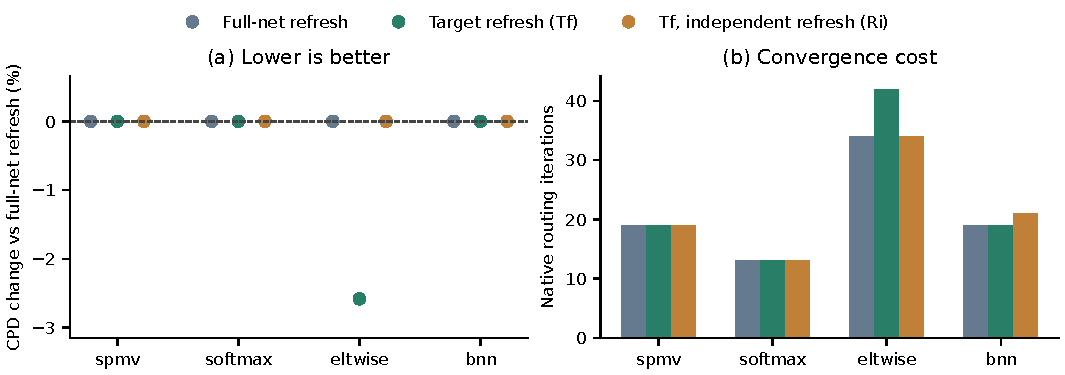
\includegraphics[width=.95\textwidth]{figures/target_feedback_ablation.pdf}
\caption{Target-refresh development evidence on four seen circuits (all plotted roles legal). The original full-net refresh is the per-circuit CPD reference. Target refresh improves eltwise timing but increases its iterations; independent refresh removes that timing gain and increases bnn iterations. Strictly matched earlier quality controls are reused. Equal CPD need not imply equal routes or resources. These single-configuration observations are not blind-test or formal runtime results.}
\label{fig:target-refresh}
\end{figure*}

A separate refresh-assignment ablation preserves the shared initial plan and replaces only finite feedback-stage solves with independent top-1 choices over the same candidate/cost construction. Its prior assignment is evaluated under that same independent objective before the unchanged 5\% hysteresis test. Candidate queries, the 128-leaf fallback, target scope, physical delays, and STA remain unchanged. This distinguishes the contribution of shared refresh planning from initial-plan differences; later routing trajectories may produce different candidate contexts. The paired eltwise experiment is sealed. Both arms share the first 87 initial tables and 110 table fingerprints in total before their trajectories diverge. The control performs 120 shared refresh solves; Ri performs 87 independent solves, with all logged old/new costs satisfying the matching-objective hysteresis rule. Ri returns to the complete original U route: CPD rises from 6.20812 to 6.37264\,ns (2.650\%), while iterations fall from 42 to 34, SB occupancy from 118 to 84, and CB occupancy rises from 955 to 972. Development planning times are 1.136390/1.161224\,s and process times 28.317328/26.815715\,s. This supports a timing-quality contribution from shared refresh planning on this case, with an iteration/resource tradeoff; it is not a global-optimality result. The unchanged-parameter independent-refresh transfer to spmv/softmax/bnn is sealed with strictly matched reused Tf quality controls. All four circuits are legal in both arms: Ri has no CPD improvement, three ties, and the eltwise regression, for a 0.656\% circuit-geometric degradation. Bnn iterations rise from 19 to 21 despite identical CPD; SB occupancy falls from 105 to 100, CB occupancy rises from 5062 to 5067, and planar wirelength falls from 2,074,317 to 2,073,244. These resource changes are not an unqualified benefit. We retain shared refresh planning for the next uniformly configured experiment. The reused transfer controls and concurrent development process times do not establish formal runtime ratios. A read-only audit of the saved failed attention route reports 232 overused resources: 231 CHANY nodes and one IPIN, none an actually used crossing entry or destination. Its reported SB/CB occupancies are 175/1630. These resources affect 442 nets with no final guides and 601 distinct descendant connections, of which 592 are same-layer and nine cross-layer. This identifies a largely unguided, same-layer congestion population; it does not prove a single-event failure cause or certify netlist endpoint mapping. The native failure remains excluded from legal CPD, and the scoped audit's existing limitations remain. The earlier selective layer-scope implementation already required a pre-prune overuse witness; that trigger is not presented as a new mechanism. The current original-scope Tf attention run also ends in native failure with the same complete failed-route body; the containing scale batch is now sealed, with this failure retained in its six-circuit denominator. The sealed combination pilot compares Tf under uniform initial-global scope against the same-scope native A1 and F1/U1 controls, with an exact U1 reproduction gate. Since A1 itself already recovers attention, any recovery under this combination cannot be attributed solely to the guide. The sealed eltwise pair regresses from 6.20393 to 6.70679\,ns (8.106\%), with SB/CB occupancy increasing from 206/1123 to 253/1156. Attention retains exactly the same complete route and 12.6638\,ns CPD in C1 and Tf1. Across these two seen cases, Tf1 degrades circuit-geometric CPD by 3.974\% against C1 and 5.567\% against same-scope native A1. Thus the original-scope Tf improvement does not transfer to this scope combination. A saved-route comparison with A1, subsequently linked to the passed batch seal and mechanism audit, identifies eight matched connections in the union of worst setup paths; none of their nets has a final guide. The largest physical RR-delay increase is on net \texttt{new\_n16746}, pin 13, from 1.035165 to 3.109805\,ns, with no layer crossing in either route. Another connection, \texttt{bram\_select[2]}, pin 2, changes from zero to two crossings and from 1.042804 to 1.696745\,ns. These are physical connection delays, not full STA increments, and do not establish the causal refresh event. The combination is not promoted. A separate guide-pressure ablation retains the same candidate construction, target refresh, and layer scope, comparing the original congestion preference weight 2 with weight 1 and a weight-0 native-equivalence diagnostic; the two-circuit batch is sealed (Table~\ref{tab:guide-pressure}). Weight 0 exactly reproduces both native A1 routes despite retaining planning. Weight 1 matches A1 CPD in both cases; on eltwise it reduces CPD from the weight-2 value by 10.269\%, lowers SB/CB occupancy from native 243/1144 to 194/1118, and uses 21 rather than 22 iterations. On attention it retains the entire weight-2 route and 49 iterations, versus native 37. Thus removing the timing regression does not yet establish a timing improvement over a strong same-scope baseline, and the resource gain coexists with a convergence penalty. Development planning/process times for weight 1 are 1.093770/26.914801\,s on eltwise and 1.899762/84.403491\,s on attention; no formal speedup is inferred. This examines indirect routing effects without increasing query budgets. A sealed decision-neutral trace exactly reproduces the weight-2 and weight-1 trajectories, including tables, refresh decisions, guides, queries, and all original non-time counters. Among 250/229 finite-table assignment events, the selected candidate has worse standalone opening-plus-branch cost than an alternative in 109/93 events, all on co-assigned candidates. The identical initial plans contribute 149 events; these repeated records are not independent samples. Therefore a leaf-local score gap would confound sharing with unreliability. A separate fixed-hierarchy exclusion diagnostic computes the optimal objective after forbidding the selected candidate for one leaf, using the two cheapest shared choices at each node and an ancestor-chain update. It has passed 20,187 exclusion comparisons on 1,000 randomized tables and sanitizer checks; the sealed native diagnostic also reproduces both complete trajectories, original counters, and local-margin records. Weight 2 has 104 strict zero-margin exclusions among 250 assignment events, including 64 of 101 accepted-refresh events; weight 1 has 76 among 229. In each trajectory, 52 locally worse selections nevertheless have positive net-level exclusion margin. Summary reconstruction and exclusion evaluation total 0.000666/0.000543\,s over 109 finite-plan events per trajectory, excluding logging; these small-case diagnostic observations are not formal production-overhead measurements. These are surrogate sensitivities, not physical-delay confidence. The exact-tie pressure ablation Z is now sealed. It changes only the extra miss weight, setting it to zero for strict finite exclusion-cost equality. Its eltwise CPD improves from 6.70679 to 6.40460\,ns, but remains 6.422\% worse than native A1; SB/CB occupancy is 217/1131 at 20 iterations. Attention exactly reproduces native A1's complete route and 37 iterations, recovering the 49-iteration penalty of the original guidance. Final zero-weight counts are 72 of 213 nominal guides on eltwise and 20 of 58 on attention. The default-off controls reproduce the original trajectories; final weights are audited from saved guide snapshots, and enabled assertions preserve non-target state. Z is not promoted.

A separate relative-sensitivity variant G uses $w=w_0\Delta/(\Delta+J_i)$ for a finite exclusion gap $\Delta$ and selected standalone opening-plus-branch cost $J_i$, with zero weight at zero gap and unchanged weight when no finite alternative exists. This introduces no fitted threshold or graph query, and is a surrogate sensitivity proxy rather than physical-delay confidence. Its sealed two-case pilot exactly reproduces both native A1 final routes and metrics, with additional planning; eltwise's median/max final coefficients are 0.0637/0.3170 and attention's 0.0826/0.1277. It provides no demonstrated QoR gain here. Combining the independently tested half-strength weight with exact-tie suppression (H) instead yields 6.59052\,ns on eltwise, 9.512\% worse than native, while attention again equals the native route. Thus the separate benefits do not combine uniformly; neither branch is promoted. These remain single-seed development observations, not formal runtime evidence.

The first fixed-parameter transfer beyond the six training circuits is sealed on seed-21 Hybrid-O/P0/W100 inputs (Table~\ref{tab:target-transfer}). Selection sorts the fourteen circuits having matching A0/R1 receipts by grid side and name, choosing \texttt{clstm\_like.small} and \texttt{conv\_layer} before new candidate outcomes were inspected. Each arm has one legal result and one routing failure. On clstm, F/V/Tf share the complete final route, 6.85706\,ns CPD, and 35 iterations; this is 1.507\% better than A0 but equal to old R1. Native initial-global A1 ties this CPD in 20 iterations with a different route. On conv, F reproduces the old R1 failed artifact, while V, Tf, and A1 also fail at 200 iterations. These failures remain in the denominator; their provisional delays are excluded from legal CPD. Tf changes 56/416 preferences on clstm/conv, all actual targets and none retained, compared with V's 148/1333 changes including 105/853 retained connections. Thus target-state preservation transfers, but additional final-quality or success gains have not appeared on these inputs. Different final guides with identical clstm routes also limit adoption-based interpretations. An invalid first launch configuration was retained separately: static F mistakenly enabled feedback-only tracing and exited before routing. Its corrected attempt uses a separate directory. The next two circuits in that pinned ordering, \texttt{robot\_rl} and \texttt{tpu\_like.small.os}, are now sealed with unchanged parameters. All F/V/Tf/A1 runs are legal on both. Robot F/V/Tf retain 13.7339\,ns and 24 iterations, whereas A1 reaches 13.3623\,ns in 17. Tpu F/V/Tf retain 7.81221\,ns, with 18/18/20 iterations and differing routes; A1 yields 7.99803\,ns in 17. Across all four transferred circuits, every arm has three legal results and one failure. Tf ties old R1 and V on all three legal CPDs; relative to A0 it has two improvements and one regression, a 0.156\% conditional geometric degradation with a 2.840\% worst tail. Relative to the different-scope A1 it has one improvement, one tie, and one regression. Thus neither feedback transfer nor uniform scope expansion establishes a general advantage here. The failures and both directions of scope tradeoff remain, without per-circuit winner selection or a blind-test claim. The weight-1 path audit also shows that CPD recovery is incomplete at the connection level: the physical delay of \texttt{new\_n16746}, pin 13, falls from 3.109805 to 1.964294\,ns, still above native 1.035165\,ns; the two-crossing detour on \texttt{bram\_select[2]}, pin 2, disappears. No single-event causal claim follows.

\begin{table*}[t]
\centering\scriptsize
\caption{Fixed-parameter seed-21 transfer. All arms are legal on clstm and fail on conv; failed CPD and legal physical occupancy are omitted. F reproduces old R1; V/Tf share its original scope, whereas A1 uses initial-global native scope. Plan/process columns are single-run development seconds, not formal speedups. Historical timing is omitted.}
\label{tab:target-transfer}
\begin{tabular}{llrrrrrr}
\hline
Circuit & Arm/state & CPD (ns) & Iter. & SB & CB & Plan (s) & Process (s) \\
\hline
clstm\_like.small & A0/legal & 6.96198 & 32 & 9 & 915 & -- & -- \\
clstm\_like.small & R1/legal & 6.85706 & 35 & 5 & 916 & -- & -- \\
clstm\_like.small & F/legal & 6.85706 & 35 & 5 & 916 & 2.544 & 46.300 \\
clstm\_like.small & V/legal & 6.85706 & 35 & 5 & 916 & 2.789 & 47.704 \\
clstm\_like.small & Tf/legal & 6.85706 & 35 & 5 & 916 & 2.642 & 47.852 \\
clstm\_like.small & A1/legal & 6.85706 & 20 & 68 & 976 & 0.000 & 41.244 \\
conv\_layer & A0/failed & -- & 200 & -- & -- & -- & -- \\
conv\_layer & R1/failed & -- & 200 & -- & -- & -- & -- \\
conv\_layer & F/failed & -- & 200 & -- & -- & 1.865 & 108.664 \\
conv\_layer & V/failed & -- & 200 & -- & -- & 3.331 & 122.995 \\
conv\_layer & Tf/failed & -- & 200 & -- & -- & 2.459 & 116.030 \\
conv\_layer & A1/failed & -- & 200 & -- & -- & 0.000 & 109.417 \\
\hline
\end{tabular}
\end{table*}


The saved conv failures provide a distinct mechanism check. Tf has 952 overused resources (951 CHANY, one CHANX); only one of its 1942 affected descendant connections has a final guide. A1 reduces overuse to 95 CHANY resources but remains stalled through iteration 200. To distinguish search failure from a necessary capacity obstruction, we enumerate every outgoing edge of the SOURCE/OPIN closure for each recorded source assignment. Let $E(N)$ be the union of first-exit RR resources for a set of distinct nets $N$. Every routed net must occupy at least one such resource, so a necessary condition is
\[
 |N| \leq \sum_{r\in E(N)} \operatorname{capacity}(r).
\]
A capacitated matching diagnostic identifies 267 nets whose complete first-exit union has capacity 172. The deficit is 95 net-occupancy units, even with no bounding-box restriction. A second implementation streams the native XML using a different parser and independently checks the source closures, every outgoing edge, capacities, and the inequality; it does not call the matching algorithm. The SOURCE assignments are identical in F/V/Tf/A1. This proves an obstruction conditional on those fixed assignments, not for alternative placements or pin mappings; no independent atom-to-terminal certification is claimed. The deficit is an excess-occupancy lower bound, not a lower bound on the number of overused nodes. A1's saved artifact has exactly 95 excess occupancy units, all within this cut. More router iterations alone cannot produce legality under these assignments, but the failure is retained in the success denominator.

The matching implementation agrees with exhaustive assignment on 503 small capacitated instances. Four independently legal routes (clstm, robot, tpu, attention) have complete first-exit matchings and constructive assignments obtained from their actual routes. The original failed attention route has the same source mapping as its legal initial-global control and also passes this necessary test. Passing therefore does not establish routability, and the cut diagnostic is not used to hide difficult inputs or replace native/independent legality checks. All failure-artifact physical counts, terminal iterations, and provisional delays remain separately archived.

The separate formal same-environment timing batch is sealed (Table~\ref{tab:formal-v14}). Five mutually legal seen circuits each receive three rotated A0/R1/U orders, yielding 45 legal roles and no gated cases. Every role passes native FULL and complete-route/quality reference equivalence; physical inputs are sealed after execution. U is the frozen full-net feedback implementation with exact closure views, preceding target-feedback, pressure, and retained-prefix experiments. With fixed CPU affinity, uniform input prewarming and no overlapping heavy study jobs, its circuit-geometric whole-process time is 21.011\% lower than old R1 but 6.246\% higher than A0. Every circuit is faster than R1 and slower than A0; U/A0 overhead ranges from 3.644\% on gemm to 7.827\% on bnn. Bnn planning falls from 268.754 to 11.020\,s and gemm from 363.257 to 28.515\,s. Bnn median peak RSS falls from 13,647,724 to 10,731,544\,KiB; memory is approximately unchanged on the other circuits. These contrasts include feedback behavior and exact reuse, so they do not isolate a cache-only causal effect. The host remains shared, the five cases were previously observed and selected for mutual legality, and attention's failure remains in the separate six-circuit quality denominator. Thus this measurement establishes reduced overhead against old R1, with residual cost against native routing; it establishes neither broader success-rate gains nor a formal runtime result for later variants. Raw repetitions, paired ratios, process maxima and GNU time counters are retained. GNU peak RSS in Linux KiB is not a simultaneous process-tree sum; rounded GNU elapsed time is separate from the full-process observer interval, and planning/router components are never added to that interval.
\begin{table*}[t]
\centering\small
\caption{Sealed same-environment timing on five previously seen, mutually legal circuits, with three rotated repetitions per arm. Full-process and planning times are per-circuit medians in seconds. U is frozen full-net feedback with exact closure views.}
\label{tab:formal-v14}
\begin{tabular}{lrrrrrrrr}
\hline
Circuit & A0 process & R1 process & U process & U/A0 & U/R1 & R1 plan & U plan & U peak RSS (GiB)\\
\hline
spmv & 17.753 & 21.210 & 19.107 & 1.076 & 0.901 & 3.301 & 1.048 & 0.993\\
softmax & 37.082 & 41.737 & 39.633 & 1.069 & 0.950 & 4.312 & 1.830 & 2.240\\
eltwise\_layer & 26.464 & 32.280 & 27.869 & 1.053 & 0.863 & 4.990 & 1.374 & 1.019\\
bnn & 263.018 & 549.419 & 283.605 & 1.078 & 0.516 & 268.754 & 11.020 & 10.234\\
gemm\_layer & 1278.617 & 1642.931 & 1325.215 & 1.036 & 0.807 & 363.257 & 28.515 & 26.256\\
\hline
\end{tabular}
\end{table*}


A further independent native search-scope experiment is registered because initial-global scope previously recovered attention even with guides disabled. It keeps the existing overuse-witness expansion and tests an additional early trigger: a native-selected net receives full layer bounds if an actual remaining target reaches criticality 0.9 after pruning and native criticality computation. XY limits, costs, routing transactions and final STA remain unchanged. Guides are disabled in the pilot. An absent trigger must reproduce original A0, and threshold zero must reproduce initial-global A1, before interpreting the 0.9 variant against both existing overuse-only and initial-global controls. This is a new timing trigger, not a re-description of the already implemented pre-prune overuse policy. The sealed eltwise pilot passes both complete-route equivalence gates and all four new routes are legal and independently audited. The 0.9 trigger expands 71 nets in the first iteration, but its 6.40159 ns CPD is worse than overuse-only expansion (6.22942 ns) and initial-global A1 (6.01810 ns), despite lower SB/CB occupancy (227/1129 versus 254/1150 and 243/1144). The unchanged-parameter attention test is also sealed and audited: K, overuse-only O and initial-global A1 all have 12.6638 ns CPD, but require 62, 31 and 37 iterations, respectively. K uses 697 SB pairs and 2297 CB sources, compared with O's 728/2329 and A1's 740/2307. Original A0 and R1 failures remain in the denominator; recovery was already achieved by both native scope controls and is not an additional success attributable to the new timing trigger. Across both development cases, K has one CPD tie and one regression against O and A1, with higher iteration counts than O. It is not promoted or combined with Tf.

Native first-legal stopping is a separate potential confounder: the default allows one legal convergence. A registered independent control permits at most two legal convergences uniformly for A0, old R1, Tf and strong full-layer A1, reusing each arm's exact immutable binary, inputs, environment and count-one result. All other router parameters remain fixed. Native selection ranks setup slack before other timing metrics and wirelength; its early-exit heuristic uses an sWNS ratio, so this experiment does not guarantee two legal convergences or minimum CPD. It will check the pre-convergence iteration prefix, actual legal cycles, best-route restoration, final STA, physical resources and complete process cost. The eltwise control is now sealed: all four count-two treatments are legal and independently audited, and every count-one iteration prefix matches through first legality. A0 improves from 9.93208 to 6.01810 ns (43 to 68 iterations) and old R1 from 6.96208 to 6.01810 ns (46 to 65). Tf remains at 6.20812 ns after 62 iterations: its second legal route has approximately 6.390 ns CPD, so the first legal route is correctly restored. Initial-global A1 retains its 6.01810 ns route and exits after one extra, infeasible iteration because the native heuristic sees no slack gain. Restored SB/CB occupancy is 30/968 for A0, 39/969 for R1, 118/955 for Tf and 243/1144 for A1. These matched native controls remove the inference that Tf's first-legal timing advantage persists with further native convergence; they are one seen development case, not a population result or formal timing comparison.

A separate default-off mechanism is registered to test whether continued guide pressure impedes this native refinement. After the first native legal convergence, it releases future per-connection guide use while retaining candidate planning and selective refresh. Physical costs, STA, search bounds, native reroute selection and transactions remain unchanged. Its disabled control must exactly reproduce count-two Tf, and its treatment must reproduce the complete printed native/planning prefix through first legality. This isolates guide use. The sealed release test passes its disabled-control, first-legal-prefix, graph/guide and input-seal gates: CPD changes from 6.20812 to 6.20393 ns, SB occupancy from 118 to 38 and CB sources from 955 to 966, with 62 to 67 iterations. The CPD gain is only 0.067492\%, and the result remains 3.087852\% worse than count-two A0/R1. It is not promoted.

An independent complementary test retains guide pressure but freezes further candidate planning after first legality. Its sealed result also passes exact disabled reproduction, initial native/planning prefix, a unique legal-phase event, unchanged subsequent plan/query/refresh counters, graph/guide audits and input sealing. CPD becomes 6.19629 ns (0.190557\% better than Tf but 2.960901\% worse than native count-two A0/R1), at 62 iterations and SB/CB occupancy 30/968. It skips 28,774 subsequent prepare calls and reduces cumulative refresh attempts from 389 to 191 and endpoint queries from 362 to 268. Paired development planning/process times are 2.320655/38.043944 s for the disabled control and 1.179399/36.079993 s for freezing; these observations require formal remeasurement before any acceleration claim. Guide use and planning freeze were tested separately and are not combined. Neither closes the CPD gap to the stronger native control. The preregistered unchanged-parameter extension on spmv, softmax and bnn is now sealed. Together with eltwise it contains 16 new legal count-two roles and 16 strictly matched, certified count-one controls; all first-legal iteration-prefix gates pass. Only eltwise changes CPD under reconvergence; spmv, softmax and bnn retain each arm's count-one CPD, although legal-cycle counts and route identity can differ. Across these four seen circuits, Tf versus old R1 changes from a 2.824838\% geometric CPD improvement at count one to a 0.780191\% regression at count two (three ties, one regression). Against count-two A0 or initial-global A1, Tf has one improvement, one tie and two regressions, with geometric regression 0.474666\% and worst regression 3.157475\%. This is a controlled seen-case result, not an independent success-rate or blind-generalization claim; original attention failures and unmeasured count-two gemm remain identified in the broader cohort. Planning, native router and complete-process costs are exported per run, without historical wall-time speedup ratios.
\begin{table*}[t]
\centering\scriptsize
\caption{Native reconvergence control on four seen circuits (one seed each). Cells show final legal CPD in ns for maximum convergence count 1 / 2. The count is an upper limit; native early exits and best-route restoration remain enabled. Failures and other statuses remain in the accompanying CSV; gemm and original attention failures are outside this four-circuit extension, not removed from the broader quality cohort.}
\label{tab:native-reconvergence}
\begin{tabular}{lrrrr}
\hline
Circuit & A0 & Old R1 & Tf & Initial-global A1 \\
\hline
eltwise\_layer & 9.93208 / 6.01810 & 6.96208 / 6.01810 & 6.20812 / 6.20812 & 6.01810 / 6.01810 \\
spmv & 7.03470 / 7.03470 & 7.04599 / 7.04599 & 7.04599 / 7.04599 & 7.03470 / 7.03470 \\
softmax & 8.97575 / 8.97575 & 8.97575 / 8.97575 & 8.97575 / 8.97575 & 8.97575 / 8.97575 \\
bnn & 13.60740 / 13.60740 & 13.42160 / 13.42160 & 13.42160 / 13.42160 & 13.60740 / 13.60740 \\
\hline
\end{tabular}
\end{table*}


A decision-neutral path-witness diagnostic reuses the settled parent forests of existing bounded delay queries, preserving the complete native route, guides, planning tables and original query work. Native C/T reproduction and an independent stream of actual RR edges, switch delays and reported price formulas pass. Replacing per-unknown trace rows with exact coverage counters retains all 26,900 measured side events among 112,704 requested events within the same 50,000 valid-record cap, with no cache or output omissions. Nevertheless, only 557 of 56,352 repeated candidate--leaf events have both sides measured; just 36 of 704 DP-proposed leaf events do, including 11 in accepted plans. These are trajectory events, not independent samples. A canonical shortest witness may miss less-congested equal-delay alternatives, and its ownership-aware negotiated multipliers are not summed native search cost. A bounded candidate-directed query is now evaluated at the same additional cap of 256 expansions per refresh. Non-directed, spatially ordered and price-aware controls obtain 0, 47 and 53 valid sink-side paths on this seen eltwise trajectory, respectively, with 672 requests in each arm; none of the new priced paths is certified optimal. All arms preserve the complete route and 6.20812 ns CPD. A separate calibrated price-score pilot uses observed bounded tolls and same-unit geometric estimates for unmeasured candidates, with reliability weighting and a two-unit cap before criticality scaling. Although it changes 4,814 branch costs and performs 48 extra shared-DP solves, independent reconstruction finds no assignment or acceptance change; the complete route and guides remain identical. The 53 observed paths do not provide two observed alternatives on any selected leaf. Of 79 scored leaf events, 75 are numerically equivalent to geometric rescaling, so this pilot provides little candidate-specific price contrast. Post-hoc matching to the complete static witness cache identifies 81 selected leaf events with at least two potential sink-side paths after pooling. These paths must be repriced under the current snapshot, since the old diagnostic multiplier sum differs from the bounded toll. The isolated cache-pooling pair is sealed: 710 existing shortest-path witnesses add current-price observations without changing any fresh query or its work. There are now 81 selected leaf events with at least two observations. Eight shared-DP proposals change, five in accepted plans, while the acceptance decisions themselves are unchanged. Two final guide preferences differ at planned criticalities 0.891 and 0.947, but neither is adopted by the unchanged physical route. Final CPD, 62 iterations and SB/CB occupancy 118/955 are unchanged. The independent audit verifies current destination-toll formulas, directed physical edges, both objective fingerprints, shared optima and prior-assignment hysteresis. Some newly preferred alternatives are unmeasured, so optimistic estimation and weak critical-connection influence remain separate hypotheses, not established causes. An independent terminal-ancestor cache compression preserves every query/path/price/table/decision record, the final guides and the full route in its sealed native pair, while reducing stored parent records from 1,482,752 to 580,273 (60.865\%). This is a cache-entry reduction, not an allocator-memory or formal runtime speedup: ordered development process times are 38.489 and 38.836 s. A separate refresh-only sink-delay test is registered with price scoring disabled. It substitutes exact cached sink distances candidate by candidate, uses per-leaf calibrated geometric estimates elsewhere and bounds signed corrections; priced-path upper bounds are excluded from exact physical calibration. The isolated price-off pair is sealed: 5,312 sink corrections comprise 710 exact cached observations and 4,602 estimates; 525 measured sink records have an unmeasured source side. Independent checks reconstruct the per-leaf median, signed cap, source/sink decomposition and 290 shared-plan objectives and fingerprints. Twenty-four proposals change, including three accepted plans, but acceptance decisions and the complete physical route remain unchanged at 6.20812 ns and 62 iterations. Three final guide preferences differ; one merely comes to agree with an already identical routed crossing. This is not a physical improvement and remains 3.157475\% worse than strong count-two native A0 and old R1 at 6.01810 ns. The next registered read-only diagnostic measures guide-only search-cost increments at actual connection criticalities before choosing a new bounded timing preference. Selected matched observations are collected in Table~\ref{tab:candidate-path-dev}.
\begin{table}[t]
\centering
\caption{Selected same-input eltwise development observations at native convergence count two. All are legal. Planning and complete-process seconds are ordered development costs, not formal speedup measurements. The physical-sink arm disables price scoring; it is not a combination claim.}
\label{tab:candidate-path-dev}
\scriptsize
\begin{tabular}{lrrrrrr}
\hline
Method & CPD (ns) & Iter. & SB & CB & Plan (s) & Proc. (s) \\
\hline
A0 & 6.01810 & 68 & 30 & 968 & 0.000 & 34.681 \\
Old R1 & 6.01810 & 65 & 39 & 969 & 4.819 & 39.643 \\
Tf & 6.20812 & 62 & 118 & 955 & 2.531 & 39.445 \\
Priced query & 6.20812 & 62 & 118 & 955 & 2.302 & 38.348 \\
Price score & 6.20812 & 62 & 118 & 955 & 2.318 & 38.186 \\
Cached price & 6.20812 & 62 & 118 & 955 & 2.356 & 38.338 \\
Compact cache & 6.20812 & 62 & 118 & 955 & 2.908 & 38.836 \\
Physical sink & 6.20812 & 62 & 118 & 955 & 2.614 & 38.638 \\
\hline
\end{tabular}
\end{table}


The historical query gate counts source-measured candidates in the ranked pool and skips a reverse query when this count is below $\min(K,|\mathrm{ranked}|)$. A preliminary global-source-empty test exercises no such contexts on this case and does not validate the historical gate. The corrected four-arm experiment crosses the actual gate with the old whole-leaf delay rule and the new partial sink rule. An independent forward Dijkstra on the actual RRG verifies 765,936 repeated candidate-availability flags over 98 source endpoints. The gate skips 651 of 853 eligible calls and reduces distinct delay queries from 362 to 185 and settlements from 1,482,752 to 757,760 (48.895\%). Under the old score, all base tables, decisions, guides and the complete route are identical. Under the new score, exact sink observations used in correction fall from 710 to 98 and branch corrections from 5,312 to 1,168; five proposals differ, including two accepted plans, and the final guides differ. Thus identical final CPD does not establish equivalence of the new scorer. All four routes nevertheless remain identical at 6.20812 ns and 62 iterations, with SB/CB occupancy 118/955. Fresh priced queries yield 67 rather than 53 valid upper-bound paths at the same 62,967 expansions, which does not replace exact physical measurements. These are development traces; their detailed candidate logging prevents a formal runtime claim. A registered lazy-query follow-up will defer reverse queries that cannot affect the old base table and resolve only leaves needed by the unchanged priority policy, requiring exact preservation of every selected-leaf query, physical score, decision and route. It has not yet been implemented or submitted. Actual search-cost influence tracing is now sealed. Enabling the read-only diagnostic preserves every original table, query, decision, native iteration counter, final guide and complete route. It observes 35,448 guided crossing evaluations, retaining 3,729 predefined stratified raw rows and exact counts for 31,719 omitted rows. Independent actual-edge/switch/configurability/physical-delay and native float multiplier checks pass on all recorded rows. On two focus connections at iteration 17, 12 and 18 crossing evaluations all miss the preferred entry; the analytical additional congestion contributions have medians 9.49 and 2.63 graph-delay units at actual criticalities 0.891 and 0.947. Thus guidance is not uniformly weak. A third connection has six guided attempts but no guided crossing evaluation; all its observed starting trees already contain re-expandable sink-layer nodes. This is present tree state, not proof of queued seeds or a unique cause.

A separate critical-cost policy preserves native congestion and replaces only the method's extra charge on configurable mismatches at actual criticality at least 0.9 with a bounded search-only timing term. Its amplitude is $\beta r d_0$, where $d_0$ is the graph delay unit and $r$ is the preferred candidates' mean half-weighted source/sink measurement coverage. Coverage is a heuristic, not a QoR probability; priced path upper bounds do not count as exact measurements. Physical delay and STA remain unchanged. The absent flag preserves the original policy, explicit $\beta=0$ removes only the critical extra, and $\beta=0.25$ adds the bounded term. Independent full-RRG bounded forward/reverse oracles validate 2,120 coverage flags over 445 endpoint/direction pairs, alongside actual cost/cap and final snapshot checks.

Stopping-rule controls reveal substantial instability (Table~\ref{tab:guide-policy-stops}). At count two the fixed term improves 6.20812 to 6.01810 ns, but its first legal, fully measured count-one result is 8.25683 ns, 33.000490\% worse than control. It ties strong count-two native A0/old R1 rather than improving them. Turning diagnostic tracing off reproduces every complete trajectory. Delaying activation until the original first-legal hook preserves the entire initial cost/query/heap prefix and count-one route, yet yields only 6.20393 ns at count two. Its zero-term refinement control has the same CPD at 76 rather than 64 iterations. A cap-only variant preserves the original operation whenever the existing analytical extra is already below the bounded term; it passes 300,000 non-amplification cases plus 200,000 compatibility cases. Nevertheless, at the quarter-unit setting its complete final routes match the fixed variant under both stopping rules, so it does not remove the first-legal regression. These variants are not promoted. A predeclared half/one-unit cap bracket will measure both stopping rules before any broader validation; it is registered, not submitted. All development costs and physical resources remain in the full evidence table, without a formal speedup claim.
\begin{table}[t]
\centering
\caption{One seen eltwise case under matched native convergence limits. CPD is final physical STA in ns; SB/CB are actual count-two net occupancies. A dash is unmeasured, not a tie. First-legal quality and later recovery are kept separate.}
\label{tab:guide-policy-stops}
\scriptsize
\begin{tabular}{lrrrrrr}
\hline
& \multicolumn{2}{c}{Count one} & \multicolumn{2}{c}{Count two} & & \\
Policy & CPD & Iter. & CPD & Iter. & SB & CB \\
\hline
Native A0 & 9.93208 & 43 & 6.01810 & 68 & 30 & 968 \\
Old R1 & 6.96208 & 46 & 6.01810 & 65 & 39 & 969 \\
Native A1 & 6.01810 & 22 & 6.01810 & 23 & 243 & 1144 \\
Original C & 6.20812 & 42 & 6.20812 & 62 & 118 & 955 \\
Critical off Z & 6.76259 & 39 & 6.38975 & 65 & 39 & 965 \\
Fixed 0.25 & 8.25683 & 57 & 6.01810 & 78 & 38 & 967 \\
Cap 0.25 & 8.25683 & 57 & 6.01810 & 78 & 38 & 967 \\
After legal: off & -- & -- & 6.20393 & 76 & 33 & 968 \\
After legal: 0.25 & 6.20812 & 42 & 6.20393 & 64 & 31 & 970 \\
\hline
\end{tabular}
\end{table}

\begin{table}[t]
\centering
\caption{Cap amplitude bracket on one seen eltwise input. Counts are native convergence limits, not repeats. Exact physical STA and actual final resource occupancies; all four roles are legal. Ordered development times are available in the bound CSV and are not formal speed ratios.}
\label{tab:cap-range}
\scriptsize
\begin{tabular}{lrrrrr}
\hline
Cap / count & CPD (ns) & Iter. & SB & CB & Plan (s) \\
\hline
0.5 / 2 & 6.01810 & 58 & 31 & 971 & 3.024 \\
1 / 2 & 6.83185 & 59 & 37 & 970 & 2.460 \\
0.5 / 1 & 8.44266 & 39 & 121 & 956 & 1.843 \\
1 / 1 & 7.85132 & 32 & 111 & 955 & 1.482 \\
\hline
\end{tabular}
\end{table}

A separately registered cap-amplitude bracket holds the router binary, inputs, endpoint budget and fresh-query cap fixed, and tests $\beta=0.5$ and $1$ under both stopping rules (Table~\ref{tab:cap-range}). All four routes pass native FULL, independent graph and final-guide checks. Independent full-RRG oracles check 468 endpoint directions and 4,242 measured-side flags; sampled native costs satisfy the local nonamplification rule. Same-amplitude first-legal prefixes reproduce across stopping rules. The half-unit cap reaches 6.01810\,ns after two convergences with 58 iterations, tying the strong native references, but its first-legal CPD is 8.44266\,ns, a 35.993827\% regression from C. The one-unit cap gives 6.83185\,ns after two convergences and 7.85132\,ns at first legality. Thus the bracket does not establish a stable candidate, and no result is selected solely from the more favorable stopping rule. Reused controls and native references are bound separately by convergence limit. A packaging failure after all native runs was recovered by checking persisted runtime/private-input digests and prior sealed controls; this recovery generated no additional route calls. Development process and planning times are retained without a formal speedup claim.

A post-hoc union of the saved worst setup paths gives 15 uniquely matched inter-cluster connections and 90 connection/result rows across the original controls and this bracket. The largest observed half-unit first-legal connection increase is 2.237549\,ns on an entirely unguided net; the corresponding one-unit example increases by 2.074640\,ns, also on an unguided net. In the earlier quarter-unit diagnostic, one such connection grows from 0.849339 to 4.402946\,ns. Exact connection delays come from independently audited physical RR traces; reported atom path increments are rounded and are not used as exact terminal certificates. These examples indicate that direct guide adoption alone cannot characterize the degradation tail. They do not identify a causal routing event or decompose the full STA difference. A separate read-only diagnostic records actual successful partial-tree seed pushes and each search's native bounding box, including high-fanout subsets and full-tree retries, before choosing a change to guide relevance. Merely observing an expandable node in a pruned tree does not prove that it was queued for that search.


This diagnostic is now sealed with exact default-off and trace-on reproduction of the full route, guides, original cost/query/heap records and physical STA. Independent native drivepoint checks cover 3,830 search rows, including 3,809 guided searches, with no search-row omissions. Of these guided searches, 2,835 actually push partial-tree sources on the sink layer. In 27 searches on five nets, no preferred crossing source/head pair passes the actual search box. A separately registered local-admission ablation suppresses only that search's preference, recomputing admission on every retry and retaining physical timing, native congestion and the saved guide state. All three roles pass native FULL, independent route/guide and input checks. Both convergence limits retain the full C route, guides, 6.20812\,ns CPD and 118/955 SB/CB occupancy. The 27 decisions are independently verified against the actual RRG and boxes. Search records change, so this is not full trajectory equivalence. This branch is not promoted; its ordered development costs are retained separately.

An offline residual-path oracle reuses all 31 fully recorded focus seed groups. It verifies actual directed zero-RC graph walks within each search box, adding the recorded seed prefix delay. All ten guided groups have a finite same-layer continuation; six have a no-new-cross physical walk no worse than the best exactly-one-preferred-cross alternative. However, four favor the extra crossing. For the critical pin-21 search at iteration 17, these physical estimates are 3.611143 versus 1.172490\,ns. Thus the mere presence of a sink-layer seed does not justify suppressing a guide. Reconstructing the existing 4,096-settlement reverse query finds only 23 of 565 repeated sink-layer seed events, motivating a fixed-budget query directed to the actual multi-source set rather than simply retaining more terminal measurements. These are physical graph-walk minima, excluding native congestion costs and possible intersections with unrecorded non-seed branches; they are not legal-extension or final-STA certificates. The offline oracle is research work, not an online overhead measurement. A multi-target residual-query comparison is registered separately before native scoring changes.

\begin{table}[t]
\centering
\caption{Read-only residual queries on one seen eltwise input: 3,809 guided searches, with 974 skipped for having no sink-layer source. Each fresh query permits 256 expansions. All modes exactly retain the original full route and 6.20812 ns CPD. Probe seconds exclude source collection and trace output; complete process costs are retained separately.}
\label{tab:residual-query}
\scriptsize
\begin{tabular}{lrrrrr}
\hline
Mode & Fresh & Paths & Hits & Expand & Probe (s) \\
\hline
Q0 & 2,835 & 687 & 0 & 725,760 & 1.306 \\
Qh & 2,835 & 1,376 & 0 & 530,656 & 1.093 \\
Qs & 1,654 & 1,595 & 1,181 & 364,731 & 0.642 \\
\hline
\end{tabular}
\end{table}

The residual-path diagnostic motivates a separately registered query experiment on the 31 saved complete seed groups. A reverse query starts at the sink and targets the actual set of queued sink-layer sources, with each source's saved prefix delay represented by a virtual analysis-terminal edge. This edge is never inserted into the RR graph. The existing generic query engine is reused with a fixed 256-expansion, 16,384-label and 65,536-heap-entry cap in both modes. A zero heuristic finds no path in these focus contexts; spatial ordering finds 13 paths, including two of ten guided contexts. All are upper bounds, with no exact certificate. Independent Floyd tests check 1,086 adapter results on 180 random small graphs and a dense storage-stop case, including zero cycles, box/layer filtering, source-as-target, absent sources and work limits. Every returned real edge and delay is independently checked against the actual RRG, and every lower or exact claim is checked against the full-distance oracle.

An offline chronological suffix pool raises coverage to 19/31 contexts and five of ten guided contexts. Reusing a prior valid suffix before querying preserves this coverage while reducing expansions from 6,843 to 4,544. The cache stores physical RR suffixes, not historical source prefix delays or prices, and checks the current source set, box and layer on lookup. These are counterfactual queries on fixed saved contexts, not native reroutes or timing measurements.

The native read-only integration reuses the existing static reverse index and preserves the complete route, guide, original planning/query/heap/prefix records and actual crossing-cost trace in all four modes (Table~\ref{tab:residual-query}). All four native roles pass FULL, independent graph, final-guide and input audits. The native coverage denominator is larger than the focus diagnostic: 3,809 guided searches, including 974 with no sink-layer source. Spatial queries return 1,376 physical walks; chronological reuse returns 1,595 and avoids 1,181 fresh queries. Expansion work falls by 31.267902\% from the spatial-only mode, with 2,012 stored witnesses and no cache or path-output stops. Independent audits check all 11,427 query attempts, 7,324 frontier lower bounds using 354 static sink/box groups and 132,634 ordinary-node settlements, 30 complete focus source sets and 20 exactly matched offline query results. Every native result remains an upper bound rather than a certified residual optimum. Full process times for C/Q0/Qh/Qs are 38.688073/39.766775/41.642259/38.391025\,s in this ordered development run. These instrumented observations establish neither a formal speed ratio nor a routing-quality improvement; final CPD remains 6.20812\,ns, still above the matched strong native 6.01810\,ns reference.

Coverage and reuse also have a quality limitation. Among 1,376 contexts with a path in both spatial-only and reuse modes, the reuse upper bound is lower in 145, equal in 1,097 and higher in 134; the largest higher-bound ratio is 2.298914. Reuse supplies 219 additional paths but does not certify a near-optimal estimate. The next registered quality hypothesis therefore requires a cached suffix to avoid every current pruned-tree node after its expandable anchor, recomputes current prefix delay and congestion prices, and tests an explicit no-new-cross alternative in the shared DP with bounded surrogate benefit and the existing refresh hysteresis. Unknown or invalid suffixes retain the original candidates. This hypothesis is registered but not implemented; a cache hit alone cannot justify removing a soft guide or changing physical timing.

The next diagnosis validates residual walks against the current pruned route tree at the existing finite-table planning points, rather than treating an old query success as a usable continuation. Both new native roles exactly retain Qs's full route, guide, original search records and non-time residual-query decisions. Independent audits cover 333 finite-table contexts, including 246 refreshes, and 853 leaf events. Among 3,663 cached witnesses, 3,544 have no anchor in the current tree, one intersects another current tree node, and 118 still extend the current tree consistently. The valid witnesses cover 106 leaf events on 11 nets; in 71 leaf events the best observed raw surrogate is below the current physical leaf's standalone cost. Of the absent-anchor records, 1,622 originate from another net, 1,589 are intermediate vertices of same-net query paths, and only 333 were previously actual expandable sources of this same net. Absence therefore cannot generally be attributed to pruning. The valid records include one cross-net witness and one former query-intermediate anchor, supporting retention of static suffixes with current-tree lookup filtering. Thus prior query coverage is a poor substitute for current-tree availability. All 3,663 witnesses match a causally prior cache insertion. Audits check 37,458 tree rows, 37,354 native float prefix-delay sums, 11,933 current-price edge snapshots and 704 independently reconstructed refresh standalone costs. The current-price formulas and within-plan snapshot consistency are verified; all-net occupancy and history-price evolution are not independently replayed. Local graph/tree consistency does not establish joint capacity feasibility or final STA improvement.

An isolated solver prototype adds an explicit per-leaf outside cost for an existing-tree continuation, opening no new crossing group. The physical candidate intersection is unchanged; an outside assignment is a distinct kind and must never index a physical RR resource. Shared and independent optima and fixed-prior assignment costs pass 1,920 checks against independent exhaustive enumeration of every cut of the fixed hierarchy on 320 random tables. There are 640 exact zero-benefit control pairs. Missing and invalid assignments, zero costs, ties and outside-only choices are included. These tests establish the surrogate solver behavior, not router integration.

The same prototype is then replayed on all 246 captured refresh tables. The original optimum, assignment, current prior cost and five-percent acceptance gate reproduce the native records, and the zero-benefit control is exact. A separately registered 25\% bound limits each outside option's modeled benefit relative to the best current physical standalone leaf cost. It changes 14 proposals and the acceptance of all 14, selecting 20 outside leaf options. These are counterfactual choices on fixed contexts; native changes would alter later trees, queries and prices. The forthcoming native quality pilot must handle intentional empty-guide metadata, same-objective prior reevaluation, invalidated anchors, non-target preservation and complete transaction/best-state restoration, then compare both first-legal and later convergence outcomes. No native quality gain is claimed from this replay.

The native outside-option pilot is now complete. The default-off build reproduces the frozen query-reuse control, and the zero-benefit mode reproduces all original cost/query/heap/prefix, guide and route records. Its original comparator initially failed because it retained 9,903 newly introduced final-state diagnostic rows; removing only this new record class yields exact old-record equality. Both completed controls were reused. The same binary and parameters then run the bounded-benefit mode under both convergence limits. All four quality/control roles pass native FULL, independent route/guide/input checks. First-legal prefixes exactly reproduce between the two limits. CPD remains 6.20812\,ns with 42/62 iterations and the same complete physical route and 118/955 SB/CB occupancy. Consequently, the inherited current-method advantage over old R1 is not an outside-DP improvement; the matched strong count-two native reference remains 6.01810\,ns.

Actual native changes are smaller than the fixed-context counterfactual. Count-two execution contains 242 refresh tables, 105 valid current-tree witnesses and seven accepted outside leaf choices in five plans. First-legal execution has 120 refresh tables and four accepted outside choices in three plans. These counts include repeated choices. Three outside leaves are present in each restored best state. All native extended costs, current-prior reevaluations, physical/outside assignments and the five-percent acceptance gate reproduce the independently tested solver on the actual captured tables. Each execution checks 9,903 best-save digests and 9,903 final digests of complete outside flag/path vectors. Two separate test-only routes each exercise one actual changed-metadata rejection: one removes newly introduced outside state, and the other restores changed pre-existing outside state. Both recover the expected snapshot digest and finish with independently checked legal routes. They are transaction diagnostics, not additional quality samples.

The bounded-benefit mode reduces guided crossing evaluations from 35,448 to 35,352, but per-iteration native routing/heap counters and the final complete route remain identical to the control. Planning/query histories do change, so full per-node trajectory equivalence is not claimed. This branch is not promoted. Ordered process times for default, zero-benefit, count-two and first-legal roles are 40.847070/41.142620/42.595828/29.223656\,s; corresponding router times are 25.29/25.04/27.08/13.79\,s, planning subitems 2.955286/2.828174/2.951390/1.544859\,s and residual-probe API subitems 0.658143/0.666044/0.655114/0.170727\,s. Subitems are not added again to router time. These detailed ordered measurements support overhead accounting, not a formal speed comparison.

The next separately registered hypothesis concerns active guide eligibility: 453 of 3,809 control guided-search events have actual criticality below the existing planning threshold. A search-local eligibility gate would preserve stored plans while testing whether stale low-criticality soft pressure matters. This is an unimplemented hypothesis, not an explanation established by the outside experiment or a reason to enlarge query budgets.

 The path-search primitive separately passes 60,000 randomized oracle checks with non-admissible ordering heuristics; only the independent minimum-pending-cost bound can certify optimality.


The smaller-credit runs also distinguish final-guide agreement from a routing improvement. On their 198 common guided connections, credits 0.25/0.5 change 20/24 preferred sets and add three guide rows each. Among the changed common connections, overlap with the final route rises from zero to 11/15, while every actual crossing set and the complete route remain unchanged. Full credit changes 23 common preferences and raises their final overlap from zero to 21, yet worsens CPD; only five of these connections change their actual crossing set. These records are independently checked final-state overlaps, not evidence that a guide caused a particular search or timing change. Source inspection further identifies a separate scoring opportunity: when bilateral delay coverage does not enable a timed leaf, the legacy branch uses a source geometry proxy with a floor of two even for expandable retained OPIN entries having zero partial-tree Tdel. A separately registered refresh-only source-delay ablation therefore substitutes current-tree Tdel divided by the existing physical unit for owned expandable source entries, including this geometry branch term, while retaining full opening costs, sink scores and native physical timing. The eltwise pilot is sealed with an exact disabled control, identical initial tables, native FULL and independent route/guide audits. Effective-source and unchanged-opening-price formulas pass on the recorded finite tables. There are 35 expandable retained entry/table records whose tree source cost differs from the geometry proxy, but only two differ from the legacy source component used in opening costs; this distinction does not certify that every associated leaf used geometry fallback. CPD worsens from 6.20812 to 7.00702\,ns (12.869\%), while iterations fall from 42 to 30. The seed-21 TPU pair is also sealed with the same validation: CPD rises from 7.81221 to 7.86071\,ns (0.621\%), while iterations fall from 20 to 18. All four new roles are legal, but both circuits lose timing quality, giving a 6.569\% circuit-geometric CPD degradation. The source variant is not promoted. Partial-tree Tdel is not an extension-delay bound.


A subsequent retained-prefix diagnostic passes default-off reproduction and trace neutrality on eltwise and seed-21 TPU, including native FULL, independent route/guide audits and input sealing. It observes 118/260 leaf events with a reachable retained crossing option among 239/303 finite-table leaf events; repeated trajectory events are not independent samples. A separate opening-cost ablation credits only the baseline component of an already owned entry during target refresh: for normalized negotiated price $p$ and credit $\alpha\in[0,1]$, the opening term becomes $s(c)+16[p-\alpha\min(1,p)]$ for owned entries, with unchanged native prices and source/branch scoring. Both default-off controls exactly reproduce frozen Tf, and initial tables match the enabled runs. All four new native roles are legal; candidate records satisfy the registered formula. Full credit ($\alpha=1$) worsens eltwise CPD from 6.20812 to 7.57905\,ns (22.083\%), iterations from 42 to 57 and SB occupancy from 118 to 181, while CB occupancy falls from 955 to 951. TPU retains its entire Tf route, 7.81221\,ns and 20 iterations despite changed planning records. Thus full ownership credit is not promoted. These cases contain no positive negotiated-premium entry records; preservation of such premiums follows from the formula rather than an observed congested-entry counterexample. Smaller credit strengths $\alpha=0.25$ and $0.5$, registered before inspecting the TPU outcome, are now sealed on eltwise with strict existing-control reuse. Both preserve the entire Tf route, 6.20812\,ns CPD, 42 iterations, and 118/955 SB/CB occupancies. Their candidate records confirm the intended discounts, so these strengths produce no final-quality or resource gain despite changed planning records. No query budget is increased; this ownership-credit branch is not promoted. This changes the surrogate objective, not physical delay or final STA, and gives no single-event explanation of the timing regression.



A decision-neutral gate diagnostic exactly reproduces Tf and reconciles 39,678 refresh contexts. Of its 191 planning attempts, 25 on 11 nets are triggered solely by non-target criticality drift; 19 are accepted, 17 without preference changes, while two preferences do change. Such events can still update metadata and are not proven redundant. A separately registered ablation restricts timing-drift eligibility to actual native targets while retaining crossing/path signals and cooldown; its sealed eltwise result retains Tf's complete route, 6.20812\,ns CPD, and 42 iterations. Attempts fall from 191 to 171, but endpoint queries rise from 268 to 277 and planning time from 1.092664 to 1.116394\,s; complete-process times are 27.770314/27.872052\,s. Final guides differ. The observed reduction in trigger count therefore establishes neither reduced search work nor a speedup, and this gate variant is not promoted.





\section{Conclusion}
Reachability-constrained shared-crossing planning provides a concrete way to coordinate vertical choices before detailed 3D FPGA routing. The evaluated static implementation produces conditional timing improvements and regressions, with substantial planning overhead and limited successful coverage. It does not establish general acceleration, universal timing superiority, or architecture-ranking reversal. The completed evidence identifies sparse delay coverage and changing critical paths as central issues, and is complemented by same-table component ablations, transactional guide feedback, query controls and exact reuse in the separate development study. Search-scope controls recover one selected failure even without guides and expose scope-dependent guide regressions, requiring a stronger matched native baseline. Post-registration development tests do not yet establish a stable improvement; the frozen evaluation remains intact.

\clearpage

\begin{table}[t]
\centering
\caption{Uniform-scope guide pressure on two seen circuits. Weight 0 retains planning but exactly reproduces the same-scope native route; it is a diagnostic, not an additional native trial. SB/CB are audited resource net occupancies.}
\label{tab:guide-pressure}
\begin{tabular}{lrrrrr}
\hline
Circuit & Weight & CPD (ns) & Iter. & SB & CB \\
\hline
eltwise & 0 & 6.01810 & 22 & 243 & 1144 \\
eltwise & 1 & 6.01810 & 21 & 194 & 1118 \\
eltwise & 2 & 6.70679 & 21 & 253 & 1156 \\
attention & 0 & 12.66380 & 37 & 740 & 2307 \\
attention & 1 & 12.66380 & 49 & 727 & 2299 \\
attention & 2 & 12.66380 & 49 & 727 & 2299 \\
\hline
\end{tabular}
\end{table}


\begin{thebibliography}{9}
\bibitem{vtr9} Verilog-to-Routing Project, ``VTR change log: v9.0.0,'' Dec. 23, 2024. [Online]. Available: \url{https://docs.verilogtorouting.org/en/latest/CHANGELOG/}. Experiments use official development revision \texttt{0b912334fdd83bb754b302146ac0d1ec9edc9a0e}.
\bibitem{vtr9paper} M. A. Elgammal et al., ``VTR 9: Open-source CAD for fabric and beyond FPGA architecture exploration,'' \emph{ACM Trans. Reconfigurable Technol. Syst.}, 2025, doi: 10.1145/3734798.
\bibitem{lazagna} I. Youssef, H. Yang, and C. Hao, ``LaZagna: An open-source framework for flexible 3D FPGA architectural exploration,'' in \emph{Proc. IEEE/ACM ICCAD}, 2025, pp. 1--9, doi: 10.1109/ICCAD66269.2025.11240893.
\bibitem{flatland} C. Hao, A. B. Kahng, B. Pramanik, and I. Youssef, ``Escaping Flatland: A placement flow for enabling 3D FPGAs,'' in \emph{Proc. ACM/IEEE DAC}, 2026, 7 pp., doi: 10.1145/3770743.3804424. Source and published CSV snapshot: \url{https://github.com/IY2002/Beyond-Flatland}, revision \texttt{84ba44acf1bad597bc5a9d1f615415870e178a86}.
\bibitem{third} A. Boutros, F. Mahmoudi, A. Mohaghegh, S. More, and V. Betz, ``Into the third dimension: Architecture exploration tools for 3D reconfigurable acceleration devices,'' in \emph{Proc. ICFPT}, 2023, pp. 198--208.
\bibitem{lazagnav1} I. Youssef, H. Yang, and C. Hao, ``LaZagna: An open-source framework for flexible 3D FPGA architectural exploration,'' arXiv:2505.05579v1, May 8, 2025, Table IV. [Online]. Available: \url{https://arxiv.org/html/2505.05579v1#S4.T4}.
\bibitem{modern} LaZagna contributors, ``VTR code port,'' source revision \texttt{5abd3acaa603e037ec390fa545b04301f13d57e0}. [Online]. Available: \url{https://github.com/IY2002/vtr-verilog-to-routing/commit/5abd3acaa603e037ec390fa545b04301f13d57e0}.
\bibitem{vtr8} K. E. Murray et al., ``VTR 8: High-performance CAD and customizable FPGA architecture modelling,'' \emph{ACM Trans. Reconfigurable Technol. Syst.}, vol. 13, no. 2, pp. 1--55, 2020.
\bibitem{h3d} Y. Zhao, F. Gu, S. Liu, P. Liao, and B. Yu, ``H3D: Heterogeneous resources aware global router for face-to-face bonded 3D ICs,'' in \emph{Proc. ICCAD}, 2025. [Online]. Available: \url{https://www.cse.cuhk.edu.hk/~byu/papers/C297-ICCAD2025-3DRoute.pdf}.
\end{thebibliography}
\end{document}
